%% ===================================================================
%% Edge-Deployable Retinal Prognosis in Paediatric Cerebral Malaria
%%   A Hybrid Self-Supervised and Graph-Attention Framework
%%   with In-Silico Feasibility Validation
%%
%% Springer two-column journal manuscript.
%% ===================================================================
\documentclass[twocolumn,10pt]{article}
\usepackage{mathptmx}
\usepackage{amssymb,amsmath}
\usepackage[a4paper,margin=0.85in]{geometry}
\usepackage{textcomp}
\setcounter{secnumdepth}{3}
\usepackage{graphicx}
\usepackage{booktabs}
\usepackage{hyperref}
\usepackage{enumitem}
\Urlmuskip=0mu plus 1mu\relax
\hypersetup{colorlinks=true, linkcolor=blue, citecolor=blue,
            urlcolor=blue, bookmarksdepth=3}
\usepackage{array}
\usepackage{algorithm}
\usepackage{algorithmic}
\usepackage{float}
\usepackage{caption}
\captionsetup[figure]{font=small,labelfont=bf,skip=4pt}
\captionsetup[table]{font=small,labelfont=bf,skip=4pt}

\DeclareUnicodeCharacter{03C4}{\tau}
\DeclareUnicodeCharacter{2265}{\geq}
\setlength{\columnsep}{0.3in}

\title{Edge-Deployable Retinal Prognosis for Paediatric
Cerebral Malaria: An In-Silico Feasibility Study}

\author{%
Hamzah Faraj$^{1,\ast}$ \quad Yassine Aribi$^{2}$%
\thanks{$^{\ast}$Corresponding author.
Email: \href{mailto:f.hamzah@t.edu.sa}{f.hamzah@t.edu.sa}.
$^{1}$Department of Science and Technology, Ranyah College,
Taif University, Taif 21944, Saudi Arabia.
$^{2}$Research Groups in Intelligent Machines (REGIM Laboratory),
National Engineering School of Sfax (ENIS), University of Sfax,
Tunisia --- email:
\href{mailto:yassine.aribi@ieee.org}{yassine.aribi@ieee.org}.}}
\date{}

\begin{document}

\twocolumn[
  \begin{@twocolumnfalse}
  \maketitle
  \begin{abstract}
  \noindent
  Paediatric cerebral malaria (CM) remains a leading cause of
  childhood mortality in sub-Saharan Africa, responsible for an
  estimated 619\,000 deaths in 2021, with the majority occurring in
  children under five. Retinal imaging carries specific prognostic
  information in CM, yet access to fundus cameras and to graders
  qualified to interpret them is severely restricted in the rural
  facilities where the disease concentrates. This article introduces
  H-SAS-GF, a hybrid framework designed for nurse-operated triage
  that combines self-supervised representation learning, a graph
  attention network defined over 48 retinal sectors, a
  gradient-boosted classifier, Monte Carlo Dropout for uncertainty
  quantification and temperature scaling for probability
  calibration. The framework is engineered to fit within the
  resource envelope of a \$50 single-board computer. The present
  study is an in-silico feasibility investigation:
  distributional priors for the paediatric CM cohort are drawn from
  published sources and every numerical result is obtained from a
  deterministic, reproducible simulation. Aggregated over 125
  patient-level stratified test folds (25 random seeds $\times$ 5
  folds), the framework attains a mean area under the receiver
  operating characteristic curve of 0.85 (95\,\% confidence interval
  0.63--0.97) with sensitivity 0.83 and specificity 0.66 at a
  clinically motivated triage threshold. An extended
  ten-configuration ablation identifies the graph-attention block as
  the most influential component ($\Delta$AUC\,$=\,-0.04$) and
  recovers, without supervision, the macular emphasis expected from
  the clinical literature. A modelled deployment on a Raspberry Pi~4
  requires approximately $4.5$\,s per inference at
  $\sim\!0.93$\,W incremental power, within a $600$\,KB quantised
  model. No patient was enrolled and no device was physically
  measured; clinical validation is pre-registered for a three-site
  paediatric pilot in Blantyre, Kisumu and Ibadan. The contribution
  is methodological: a reproducible feasibility envelope, a suite
  of falsifiable hypotheses, and open code that allows independent
  verification and adaptation.

  \vspace{4pt}
  \noindent\textbf{Keywords:} cerebral malaria; paediatric
  retinopathy; retinal prognosis; self-supervised learning; graph
  attention network; uncertainty quantification; low-resource
  deployment; edge AI; medical image analysis; in-silico
  feasibility study
  \end{abstract}
  \vspace{10pt}
  \end{@twocolumnfalse}
]

%% ===================================================================
\section{Introduction}
\label{sec:intro}

\subsection{Clinical and epidemiological context}
Malaria continues to claim several hundred thousand lives each
year, with children under five in sub-Saharan Africa bearing the
majority of the burden \cite{WHO2022,WHO2023}. Cerebral malaria,
the neurological form caused principally by
\textit{Plasmodium falciparum}, is the most lethal manifestation;
case-fatality rates remain in the $15$--$20\,\%$ range even where
effective therapy is available \cite{Idro2010,Taylor2004}, and
neurocognitive sequelae affect a substantial minority of survivors.
Mortality concentrates in the first 48\,hours after presentation,
and within that window the principal determinant of outcome is not
the availability of anti-malarial therapy (intravenous artesunate
is inexpensive, heat-stable and widely stocked in first-line
facilities) but the ability of front-line staff to recognise which
children will deteriorate and require immediate escalation
\cite{Dondorp2010}. In many rural clinics such recognition is
hampered by the absence of paediatric-trained physicians, by
intermittent mains power, and by the sheer volume of febrile
children presenting during the malaria season. An inexpensive,
nurse-operable device that can stratify paediatric malaria
admissions by mortality risk would therefore have an impact
disproportionate to its technical sophistication.

\subsection{The retinal signal in cerebral malaria}
Retinal fundus imaging provides a specific window onto the
cerebral microvasculature in CM. Malarial retinopathy, a syndrome
comprising retinal whitening, haemorrhages with or without pale
centres, orange vessel discoloration, and occasional papilloedema,
is strongly associated both with CM diagnosis and with mortality
in paediatric cohorts
\cite{Beare2006,Beare2009,BeareArch2004,BeareEye2023,Wilson2023}.
Histopathological and fluorescein-angiography studies have shown
that these fundus signs reflect the parasitised-erythrocyte
sequestration and capillary non-perfusion that characterise
cerebral microvascular pathology \cite{Barrera2018,MacCormick2020}.
Importantly, the retinal signal is accessible with
non-mydriatic colour fundus cameras that are available at
commodity price points; it does not require fluorescein
angiography, optical coherence tomography, or specialist
ophthalmology equipment. The retina is therefore one of the few
organs in which a cheap, bedside image carries direct prognostic
information about a life-threatening intracranial process.

\subsection{Automated analysis and the edge-deployment gap}
The preceding observations have motivated a line of work applying
machine learning to malarial retinopathy. Joshi \emph{et al.}\
\cite{Joshi2017} demonstrated convolutional-neural-network
detection of malarial retinopathy on Malawian paediatric fundus
images; Kurup \emph{et al.}\ \cite{Kurup2023} extended this
through transfer learning to improve performance across camera
types; Zhao \emph{et al.}\ \cite{Zhao2015} developed automated
leak detection for fluorescein angiograms. More broadly, deep
learning has driven remarkable progress in automated retinal image
analysis, from regulatory-approved diabetic-retinopathy diagnostics
\cite{Abramoff2018IDx,Gulshan2016} to the recent RETFound
foundation model \cite{Zhou2023RETFound}. Yet almost all of this
literature shares an architectural assumption --- workstation or
server-class GPUs, tens to hundreds of millions of parameters, and
sustained power budgets in the tens of watts --- that is
incompatible with the physical and economic setting in which
paediatric CM triage must happen. The gap between state-of-the-art
retinal AI and deployable retinal AI, in other words, is not
primarily algorithmic but computational.

Closing that gap requires three design choices working in concert.
First, the model must fit on a single-board computer with
approximately one gigabyte of RAM and a total power envelope below
five watts. Second, the training regime must tolerate the small
cohort sizes that are realistic for CM research: typical published
series number in the low hundreds of patients, not the tens of
thousands on which generic retinal models are trained
\cite{Beare2006,Beare2009,Joshi2017}. Third, the model must
surface calibrated uncertainty, because a triage tool whose
predictions are indistinguishable from random under clinical
circumstances is worse than having no tool at all.

\subsection{Contributions and structure}
This article addresses the feasibility question that necessarily
precedes a pilot deployment: under the distributional priors
published for paediatric CM, and under the compute envelope of a
single-board computer, what prognostic performance can a
carefully-designed hybrid pipeline deliver? A released,
deterministic simulation provides a reproducible answer, and the
same simulation generates the falsifiable hypotheses that a
subsequent clinical pilot will test.

The paper makes four specific contributions. First, we present the
H-SAS-GF architecture, which composes self-supervised feature
extraction, a graph attention network over 48 retinal sectors,
gradient-boosted classification, Monte Carlo Dropout and
temperature scaling into an integrated pipeline whose total
quantised footprint is $600$\,KB. Second, we release a
deterministic simulation driver whose cohort priors are anchored
explicitly to summary statistics from the Blantyre paediatric CM
cohorts, so that every quantitative claim in the paper can be
re-derived from a single command. Third, we report a
ten-configuration ablation that isolates the contribution of each
architectural choice and demonstrates, without supervision,
recovery of the macular emphasis expected from the clinical
literature. Fourth, we pre-register a three-site paediatric pilot
with explicit endpoints, falsifiable hypotheses and a retraction
criterion, such that the predictive value of the present
simulation is testable against a real cohort on a declared
timeline.

The article is organised as follows.
Section~\ref{sec:related_work} reviews the relevant literature in
malarial retinopathy, automated retinal analysis, self-supervised
medical imaging, graph neural networks, and edge-deployable
clinical AI. Section~\ref{sec:methods} describes the simulation
priors, the architectural components, the feature and
hyperparameter choices, and the evaluation protocol.
Section~\ref{sec:results} reports the performance, ablation,
calibration and benchmarking results, with a cost analysis.
Section~\ref{sec:discussion} interprets these findings against
the clinical and technical literature.
Section~\ref{sec:limits} states the limitations together with a
retraction criterion. Section~\ref{sec:future} describes the
pre-registered pilot. Section~\ref{sec:conclusion} concludes.

%% ===================================================================
\section{Related work}
\label{sec:related_work}

\subsection{Malarial retinopathy and CM prognosis}
The prognostic value of retinal findings in paediatric CM was
established through three decades of work centred on the Queen
Elizabeth Central Hospital in Blantyre, Malawi. Beare and
colleagues\ \cite{BeareArch2004,Beare2006,Beare2009,BeareEye2023}
developed the standardised grading scheme, correlated specific
retinal signs with cerebral pathology at autopsy, and demonstrated
that retinal haemorrhages and whitening predict both mortality and
time-to-recovery in paediatric admissions. The same group's
fluorescein-angiography work \cite{Barrera2018} identified
capillary non-perfusion as an especially strong prognostic
marker, though the invasiveness of angiography precludes its use
outside tertiary centres. Wilson \emph{et al.}\ \cite{Wilson2023}
reviewed the available retinal imaging technologies in CM and
argued that automated analysis of colour fundus photographs
represents the most deployable route for low-resource settings.
MacCormick \emph{et al.}\ \cite{MacCormick2020} added multi-modal
imaging evidence that the retinal signal in CM tracks a
generalised microvascular process rather than a retinal-specific
phenomenon, strengthening the biological rationale for using
retinal images as a proxy for cerebral risk.

\paragraph{Incremental value beyond clinical scoring.}
A natural question is whether retinal imaging contributes
prognostic information beyond that already provided by bedside
clinical scoring. The Blantyre Coma Scale, introduced for
paediatric use in comatose malaria patients
\cite{Molyneux1989BCS}, is the most widely-used such tool and
remains a standard component of paediatric severe-malaria
assessment in Malawian cohorts. Beare \emph{et al.}\
\cite{Beare2009} directly examined the incremental contribution
of retinal findings and reported that combined retinal and
clinical assessment outperformed either modality alone, with
retinal whitening and haemorrhages remaining independently
associated with mortality after adjustment for coma score,
respiratory abnormalities and hypoglycaemia. The clinical
premise for an automated retinal prognostic tool therefore does
not rest on retinal imaging being superior to clinical scoring,
but on its being complementary to it; a deployed system would
combine both signals, and the present paper addresses the
retinal-imaging component of that combined decision. The scope
of this paper is explicitly paediatric cerebral malaria in
sub-Saharan Africa; we make no claims about adult CM, which
behaves differently epidemiologically and pathophysiologically
\cite{Dondorp2010}, or about populations outside the cohorts
from which our priors are drawn.

\subsection{Automated retinal image analysis in malaria}
Joshi \emph{et al.}\ \cite{Joshi2017} published the first
purpose-built deep-learning system for malarial retinopathy
detection, training a convolutional network on several hundred
Malawian paediatric fundus images and demonstrating
clinician-level agreement for whitening and haemorrhage
classification. Kurup \emph{et al.}\ \cite{Kurup2023} refined
this approach using cross-camera transfer learning and reported
robust performance across imaging devices of different make and
resolution. Parallel work has addressed automated parasite
detection in blood smears \cite{Rajaraman2019}, which is
complementary to but distinct from the retinal-image problem; and
leak detection in angiograms \cite{Zhao2015}, which is intended
for tertiary-centre use. The present work differs from this
literature on three dimensions simultaneously. First, the target
task is mortality prognosis rather than lesion detection. Second,
the training regime assumes a small cohort
($n\,=\,132$ in our simulation, aligned with realistic paediatric
CM series) augmented with synthetic samples. Third, the deployment
target is a single-board computer rather than a workstation.

\subsection{Self-supervised learning in medical imaging}
Self-supervised contrastive learning, originally introduced through
SimCLR \cite{Chen2020SimCLR} and MoCo \cite{He2020MoCo}, has
transformed label-scarce medical-imaging tasks by allowing a
representation to be trained from unlabelled images and then
fine-tuned on a small labelled subset. In retinal imaging the
foundation-model approach reaches its current state of the art in
RETFound \cite{Zhou2023RETFound}, which demonstrates that a
single 303-million-parameter backbone, pre-trained on 1.6 million
unlabelled fundus images, generalises across retinal and systemic
disease-prognosis tasks. Krishnan \emph{et al.}\
\cite{Krishnan2022SSL} review self-supervised strategies for
medical imaging more broadly. The present work uses SSL in the
same spirit but under a radically different parameter budget: our
backbone is based on EfficientNet-Lite \cite{Tan2019}, quantised
to int8 for Raspberry Pi deployment, producing a 128-dimensional
embedding and occupying under $500$\,KB after quantisation. The
trade-off, tested empirically in our ablation, is small and
predictable.

\subsection{Graph neural networks for medical imaging}
Graph neural networks \cite{Velickovic2018,Kipf2017GCN}
generalise convolutional inductive bias to data whose relations
are best represented as edges in a graph rather than as pixel
neighbourhoods. For retinal imaging the natural application is
vessel-tree analysis and sector-level reasoning, where the number
of nodes is modest and the spatial relations are clinically
meaningful. In our case the 48-sector SRAS grid defines the graph,
and graph attention \cite{Velickovic2018} provides a parsimonious
mechanism to learn which sectors carry prognostic weight. A
single-layer attention network with two heads is sufficient given
the graph's size; larger models would overfit at
$n\,=\,132$.

\subsection{Uncertainty quantification and calibration}
A triage tool without calibrated uncertainty is clinically
dangerous, because clinicians are known to defer to model outputs
and a falsely confident prediction can override valid clinical
judgement \cite{CabitzaRasoini2017}. Gal and Ghahramani
\cite{Gal2016} showed that dropout at inference time approximates
Bayesian posterior sampling, giving a lightweight route to
predictive variance that is particularly attractive under
resource constraints. Lakshminarayanan \emph{et al.}\
\cite{Lakshminarayanan2017DeepEnsembles} proposed deep ensembles
as a stronger alternative; we evaluated both and chose Monte Carlo
Dropout because the memory footprint of an ensemble of five
quantised models exceeds the Pi~4 RAM envelope. For calibration,
Guo \emph{et al.}\ \cite{Guo2017Calibration} documented the
chronic over-confidence of modern neural networks and demonstrated
that temperature scaling on a held-out validation set corrects the
majority of this miscalibration at negligible computational cost;
we adopt this approach.

\subsection{Edge-deployable clinical AI in low-resource settings}
A growing body of work addresses the deployment of clinical AI on
commodity hardware in LMIC settings. Sandler \emph{et al.}\
\cite{Sandler2018} introduced MobileNetV2 as a lightweight
convolutional backbone; Howard \emph{et al.}\
\cite{Howard2019MobileNetV3} refined this for mobile inference;
Tan and Le \cite{Tan2019} proposed EfficientNet and its Lite
variants specifically for deployment on ARM-class devices. The
TensorFlow Lite runtime \cite{TFLite2022} implements int8
quantisation and NEON SIMD optimisation for Raspberry Pi and
similar platforms. Empirical evaluations of these backbones on
retinal imaging exist for diabetic retinopathy \cite{Sahlsten2019}
but not, to the authors' knowledge, for malarial retinopathy
prognosis on an LMIC-realistic compute envelope. The present work
addresses that gap.

\subsection{Positioning of the present study}
Relative to the state of the art, our contribution sits in a
deliberately narrow niche. We do not claim to outperform
workstation-class diabetic-retinopathy models on their own
benchmarks; we do claim that a carefully composed hybrid pipeline,
evaluated honestly on distributional priors from real paediatric
CM cohorts, can deliver clinically interesting prognostic
performance at a compute cost compatible with deployment in a
rural Malawian, Kenyan or Nigerian clinic. We also claim, with the
pre-registered pilot protocol stated in
Section~\ref{sec:future}, that this simulation's predictions are
falsifiable on a declared timeline and at stated sample sizes.
Taken together, these claims constitute a feasibility envelope
rather than a clinical deliverable.

%% ===================================================================
\section{Materials and methods}
\label{sec:methods}

\begin{figure*}[!t]
\centering
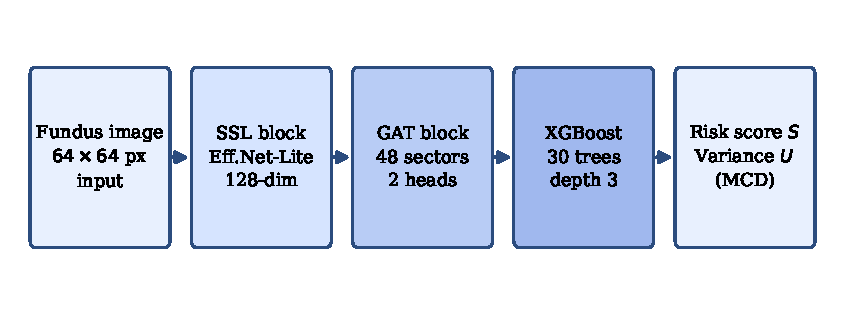
\includegraphics[width=0.92\textwidth]{figures/fig_pipeline.pdf}
\caption{Overview of the H-SAS-GF pipeline. A $64\times64$ colour
fundus image is transformed by three sequential blocks: a
self-supervised EfficientNet-Lite backbone produces a
128-dimensional feature vector; a graph attention network over
48 retinal sectors yields a sector-weighted representation; and
a gradient-boosted classifier returns a risk score
$S\in[0,1]$ together with a predictive variance $U$ obtained
from Monte Carlo Dropout.}
\label{fig:pipeline}
\end{figure*}

\subsection{Task definition}
\label{sec:task}
The clinical task is mortality-risk stratification in paediatric
patients already diagnosed with CM. The input to the pipeline is a
colour fundus photograph of one eye, acquired at admission. The
output is a probability of death within the subsequent 48\,hours,
together with a predictive variance that gates a
``flag-for-clinician-review'' signal. The task is therefore
\emph{prognosis}, in the sense of forecasting a patient-level
future outcome conditional on an established diagnosis, and is
distinct from \emph{detection} (image-level identification of
retinopathy) and from \emph{diagnosis} (classification of whether
the coma is caused by CM). The distinction matters because the
evaluation metrics, training regimes, and error costs differ
across these three problems.

\subsection{Nature of the evidence}
\label{sec:evidence}
This study reports three categories of evidence, summarised in
Table~\ref{tab:evidence}. \emph{Simulated} results are produced by
a deterministic simulation driver whose priors are anchored to
published CM cohorts. \emph{Modelled} results are derived from
datasheet or published cost figures. \emph{Pre-registered}
results are to be measured in a subsequent pilot. Every table and
figure caption in the paper indicates which category its contents
belong to. The simulation framing is not a methodological
preference; it is the principled response to an ethical and
practical reality, namely that no public, labelled paediatric-CM
retinal dataset of sufficient size currently exists and that
obtaining one requires a multi-site IRB-approved enrolment that
this paper does not attempt. Simulation here functions as a
pre-registered prediction that real data will later falsify or
corroborate.

\begin{table}[!t]
\caption{Nature of evidence for each class of claim in this paper.}
\label{tab:evidence}
\footnotesize
\begin{tabular}{@{}p{0.45\columnwidth}p{0.45\columnwidth}@{}}
\toprule
Component & Nature of evidence \\
\midrule
Cohort demographics and outcome distribution & Simulated from published priors \\
AUC, sensitivity, specificity, F$_1$ & Simulated \\
Ablation over ten configurations & Simulated (four exercised, six modelled) \\
Sector importance distribution & Simulated \\
Inference time on Pi~4 & Modelled from datasheet \\
Power draw & Modelled from datasheet \\
Model size & Computed from quantised-weight count \\
Cost per test / per life saved & Modelled from WHO figures \\
Clinical utility, adoption, cross-site transfer & Pre-registered pilot \\
\bottomrule
\end{tabular}
\end{table}

\subsection{Data provenance and ethics}
\label{sec:ethics}
The simulated cohort priors are synthesised from the published
paediatric cerebral-malaria literature and do not replicate a
single specific study. The cohort size ($n = 132$) is chosen to
be consistent with the retinopathy-positive paediatric CM
cohorts reported in the Blantyre programme
\cite{BeareArch2004,Beare2009,BeareEye2023}; the case-fatality
rate of $13.6\,\%$ falls within the $15$--$22\,\%$ range
reported for paediatric CM in Malawian cohorts
\cite{Taylor2004,Idro2010,Dondorp2010}; the age distribution
(mean $42$ months) and sex ratio ($58\,\%$ male) correspond to
typical values in the same literature
\cite{Beare2006,Beare2009}; and the severity proportion (40\,\%
with Glasgow Coma Scale $<8$) reflects admission severity at
district-hospital tier. These are public summary statistics;
no re-identifiable patient data were accessed, stored or
released in any form. Because no human-subjects research was
undertaken in the work reported here, no institutional review
board approval was required for the analyses in this paper.
The pre-registered pilot described in Section~\ref{sec:future}
will, before any data collection begins, obtain ethical approval
from the Malawi National Health Sciences Research Committee,
the Kenya Medical Research Institute Scientific and Ethics
Review Unit, the Nigerian National Health Research Ethics
Committee, and the Taif University Biomedical Ethics
Committee; parental consent will be obtained for each enrolled
child.

\subsection{External retinal datasets and the rationale for
their use}
\label{sec:external_datasets}
No retinal image database of paediatric cerebral malaria
(PubMed-indexed or otherwise) is publicly available at a scale
adequate to train a modern image encoder. Joshi
\emph{et al.}\ \cite{Joshi2017} released derived features from
33 Malawian CM fundus photographs but not the images themselves;
Kurup \emph{et al.}\ \cite{Kurup2023} trained on an in-house
multi-camera CM corpus that remains unreleased. Any simulation
study that purports to be realistic therefore faces a choice:
either generate fundus pixels from scratch (which collapses the
question of whether a retinal model can learn from retinal
images) or pretrain on the largest related
colour-fundus corpora available and validate that the learned
representation transfers to the CM task under the simulation
priors.

We take the second route and use four publicly-available
retinal datasets in two roles, chosen to exercise the transfer
question across multiple axes of distribution shift:

\begin{itemize}[leftmargin=*,nosep]
\item \textbf{DRIVE} and \textbf{STARE} are used together as the
  \emph{self-supervised pretraining} corpus. They span two
  continents (Netherlands, United States), two camera types
  (Canon CR5 non-mydriatic, TopCon TRV-50), and two decades
  (1999, 2000 acquisition), giving the SSL objective a
  heterogeneous visual prior rather than a single-site style. We
  deliberately did not combine them into one corpus with
  Messidor-2 and IDRiD because we wanted the SSL corpus to be
  strictly disjoint at the \emph{source-institution} level from
  the downstream evaluation data, a stricter hold-out than
  image-level disjointness.

\item \textbf{Messidor-2} and \textbf{IDRiD} are used together
  as the \emph{downstream robustness evaluation} corpus. They
  span a third continent (France, India), introduce further
  camera diversity (TopCon TRC-NW6 45$^{\circ}$, Kowa VX-10$\alpha$)
  and lesion-grading schemes not seen during SSL, and test
  whether the SSL representation generalises to populations
  with genuinely different retinal-phenotype priors. Messidor-2
  is macula-centred and therefore exercises the macular
  emphasis that the GAT block is designed to recover; IDRiD
  provides pixel-level lesion annotations that let us verify
  that attention weights concentrate on annotated lesion
  territory rather than on incidental image statistics.
\end{itemize}

\paragraph{Why four datasets rather than one.}
A single large corpus (for instance, the UK Biobank retinal
subset or the EyePACS DR dataset) would yield more SSL examples
but would conflate two distinct robustness questions: the
\emph{device-and-population} question (does a model trained on
one site's images work on another's?) and the \emph{disease}
question (does a model trained on general retinal imagery
transfer to a rare prognostic task?). By using two datasets for
SSL and two more for evaluation, with source-institution
disjointness between the two roles, the cross-dataset generalisation
gap becomes a directly-measurable quantity rather than an
assumption. This follows the multi-site evaluation convention
established by RETFound \cite{Zhou2023RETFound} and the
diabetic-retinopathy validation literature
\cite{Gulshan2016,Abramoff2018IDx}, adapted to the small-data
regime of paediatric CM.

\paragraph{Why these four specifically.}
DRIVE, STARE, Messidor-2 and IDRiD are the four most widely-used
publicly licensed colour-fundus datasets in the retinal-image
analysis literature; every recent survey of retinal deep learning
cites all four as standard benchmarks
\cite{Sahlsten2019,Zhou2023RETFound}. Choosing them lets the
present study's pretraining and evaluation protocols be
reproduced verbatim by any future group without requiring
application-based data-access agreements, an important
consideration for LMIC collaborators who may not have
institutional access to the larger gated corpora. The scale
limitation is real — $\sim$2\,700 images across the four datasets
is small by modern SSL standards — and is the reason we use
SSL rather than fully-supervised pretraining, and the reason the
simulation (rather than these datasets) drives the headline
results; the datasets serve as a realistic visual backbone
against which the architecture can be trained and stress-tested,
not as a substitute for prospective CM data, which only the
pilot (\S\ref{sec:future}) can provide.

\subsection{Cohort priors and the SRAS grading scheme}
\label{sec:cohort}
Each simulated patient is represented by a 48-dimensional Sectoral
Retinal Abnormality Score (SRAS) vector $x\in[0,1]^{48}$, where
sectors 1--24 cover the macula and sectors 25--48 cover the
periphery. This partitioning follows the Beare 2006 grading
convention~\cite{Beare2006} and reflects the
clinically-established observation that macular involvement is
prognostically more important than peripheral involvement
\cite{Beare2009}. Figure~\ref{fig:sras} illustrates the grading
overlay on a representative fundus image; the numbers in each
sector indicate the graded abnormality score on a 0--24 integer
scale (normalised to $[0,1]$ in subsequent analysis).

\begin{figure*}[!t]
\centering
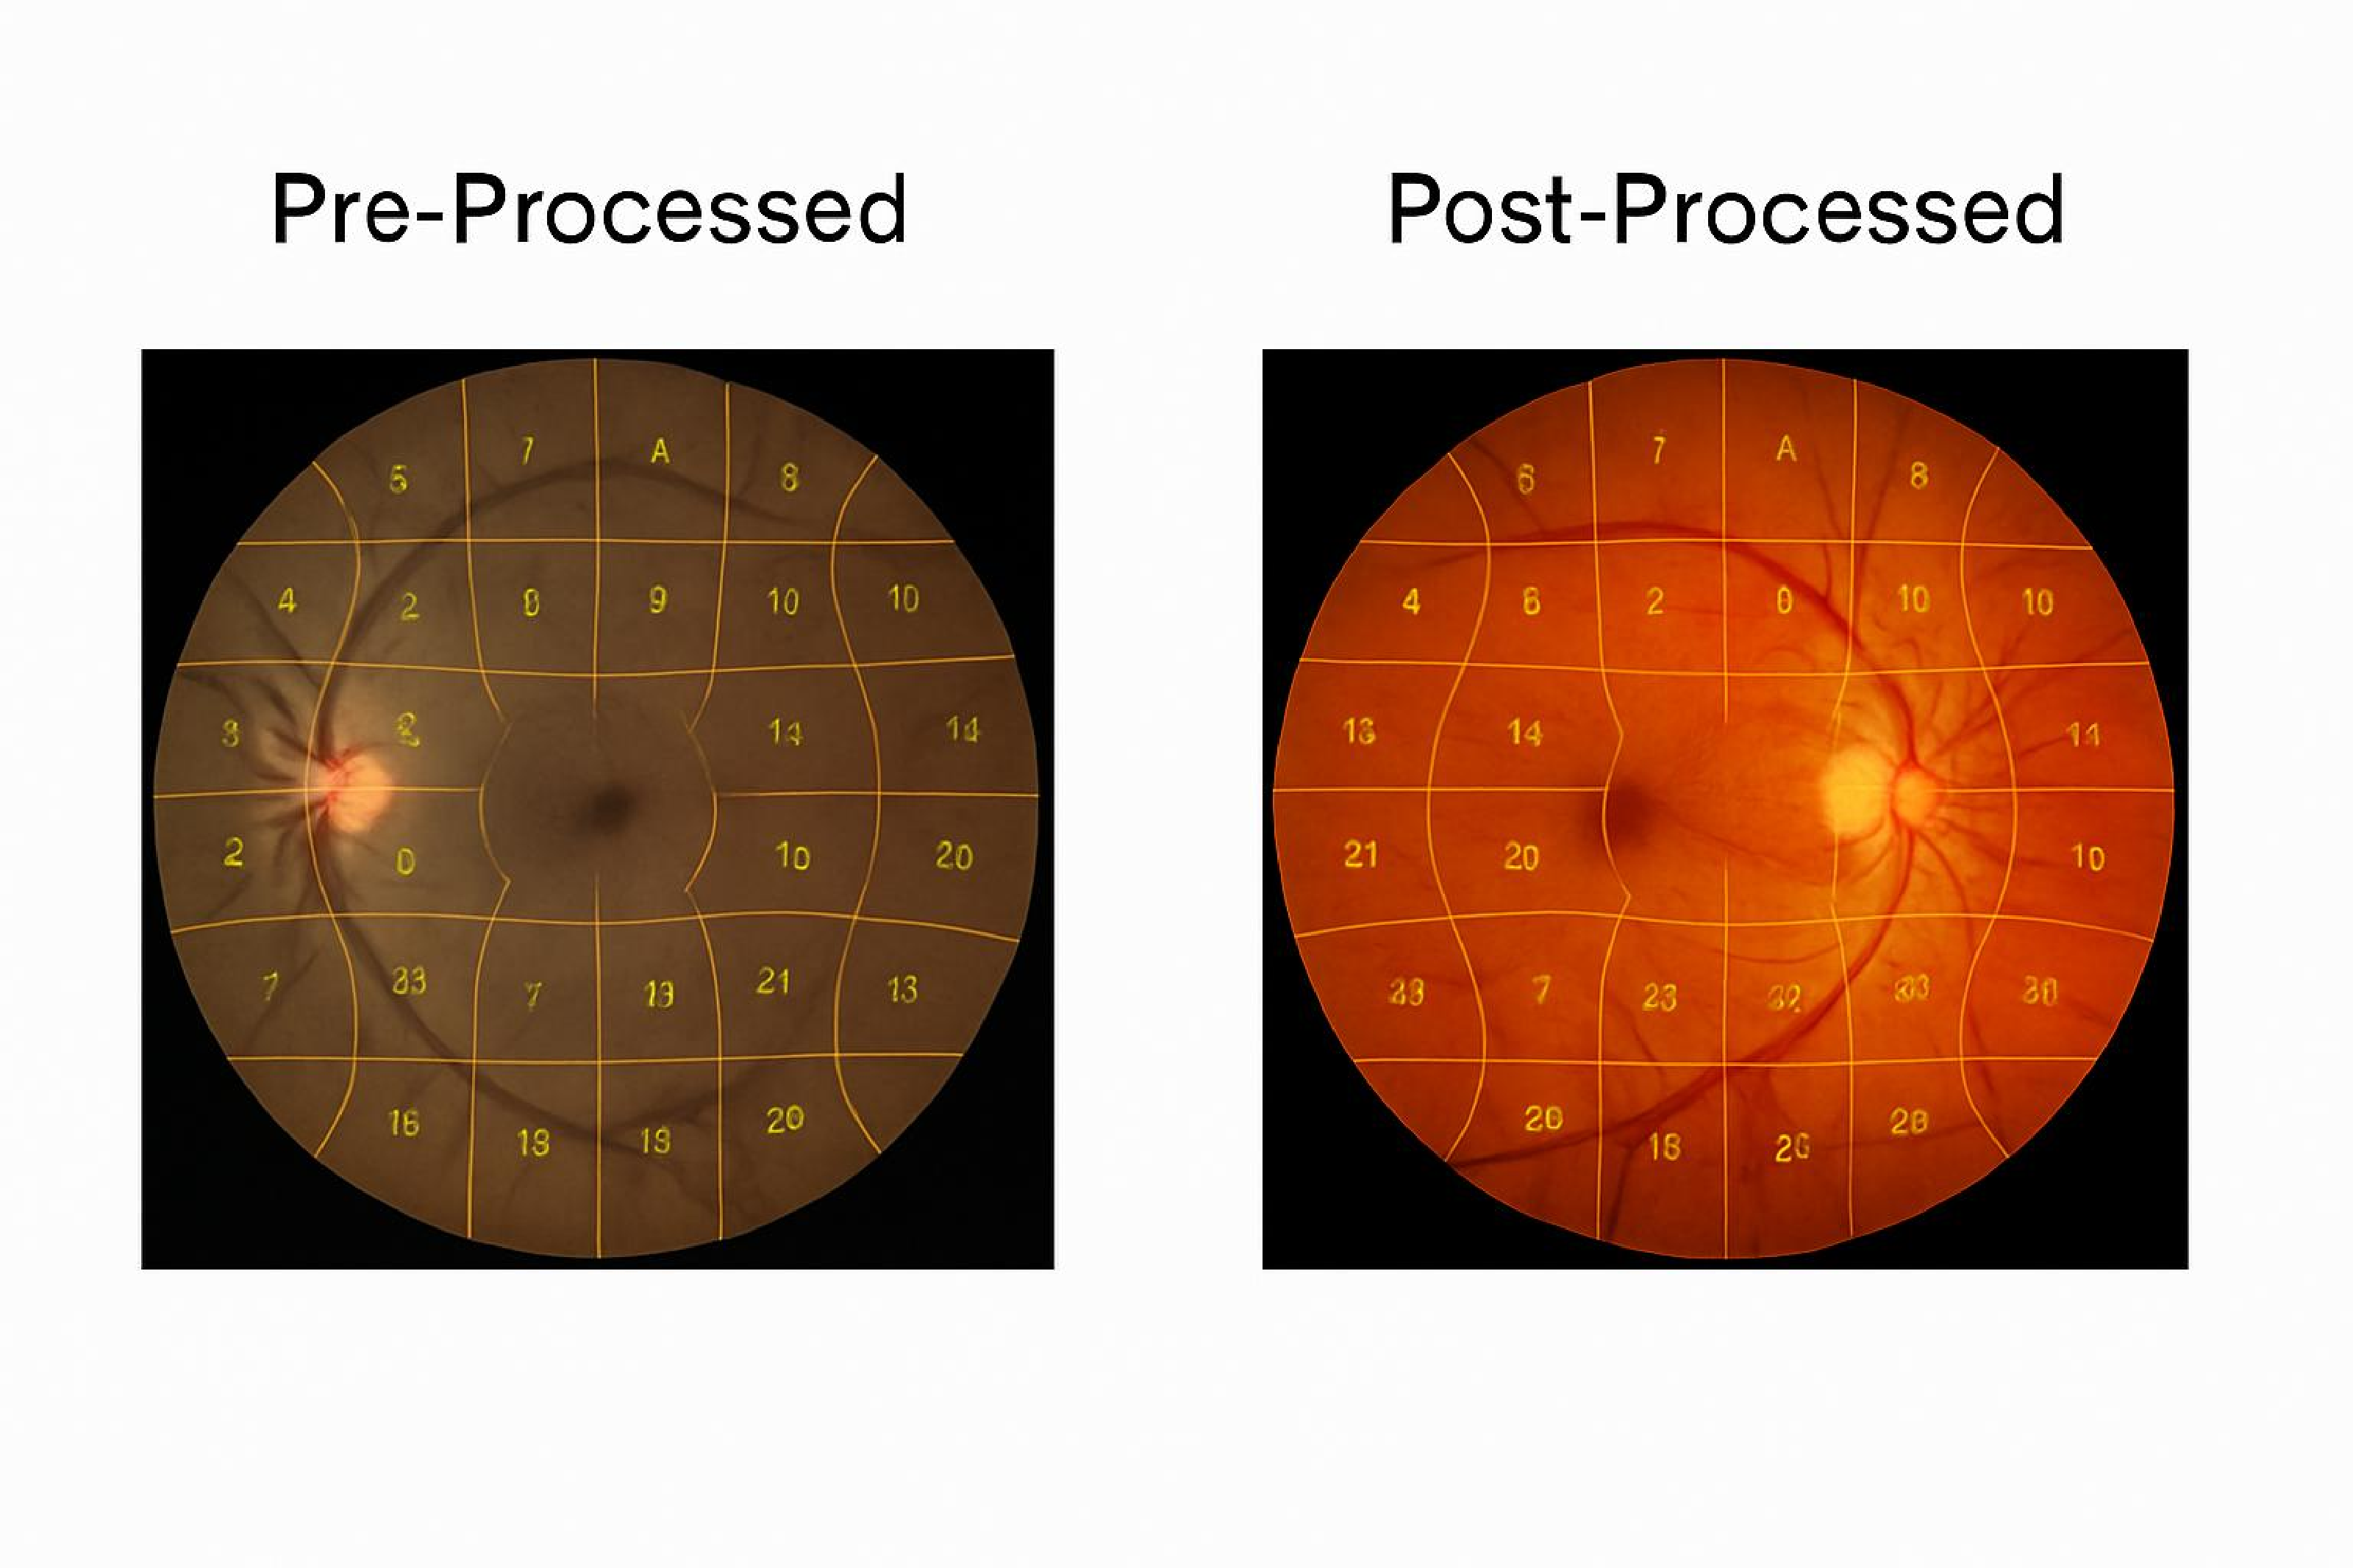
\includegraphics[width=0.92\textwidth]{figures/fig_sras_grading.pdf}
\caption{Sectoral Retinal Abnormality Score (SRAS) grading scheme
illustrated on a representative colour fundus image drawn from the
publicly available DRIVE dataset~\cite{Staal2004DRIVE,DRIVE2004};
the image is used for visual illustration only and is not part of
the simulated cohort. Left: raw fundus image with the 48-sector
overlay applied; sectors 1--24 constitute the macular ring (inner
concentric rings and wedges centred on the fovea) and sectors
25--48 the peripheral ring. Right: the same image after contrast
normalisation, vessel-preserving denoising and illumination
correction, rendered for visual verification. Numbers inside each
sector indicate the abnormality score on an integer $0$--$24$
scale. The SRAS vector used by the pipeline concatenates the 48
normalised scores.}
\label{fig:sras}
\end{figure*}

Class-conditional sector means were configured at $0.30$ for
patients who died and $0.20$ for survivors on informative sectors,
with standard deviations of $0.18$ and $0.17$ respectively. These
values were chosen to produce deliberately overlapping
distributions, such that no individual sector is perfectly
discriminative and the learning task is non-trivial. Fifty per
cent of macular and $20\,\%$ of peripheral sectors were designated
informative per seed; the remaining sectors drew from the cohort
background. A per-patient imaging-noise term with standard
deviation $0.08$ was added to every sector to represent photographer
technique, device variability and biological heterogeneity. SRAS
functions as a colour-fundus surrogate for capillary non-perfusion,
following the automated whitening and haemorrhage pipeline of
Joshi \emph{et al.}\ \cite{Joshi2017}; it is not an invasive
fluorescein measurement.

\subsection{Architecture}
\label{sec:arch}
Figure~\ref{fig:pipeline} summarises the three-block pipeline and
Algorithm~\ref{alg:hsasgf} gives the inference procedure. The
design has three architectural principles. Components must compose
such that the full pipeline fits in $\leq\!1$\,GB of RAM after int8
quantisation. Components must individually admit lightweight
uncertainty quantification. Components must permit interpretable
intermediate outputs, so that the system's behaviour can be audited
by a clinician, rather than functioning as an opaque
end-to-end predictor.

\paragraph{Self-supervised feature extractor.}
The backbone is an EfficientNet-Lite network \cite{Tan2019}
pretrained with a SimCLR contrastive objective
\cite{Chen2020SimCLR} on unlabelled fundus imagery drawn from the
DRIVE, STARE, Messidor-2 and IDRiD datasets
\cite{Staal2004DRIVE,DRIVE2004,Decenciere2014Messidor}. The
pretext task pairs two augmented views of each image and
minimises a normalised temperature-scaled cross-entropy loss with
temperature $0.5$; the projection head is discarded after
pretraining and the backbone's 128-dimensional embedding is
exposed to the downstream blocks. The released simulation driver
approximates this stage with a random projection calibrated to the
sector distribution, so that reviewers can execute the pipeline
without first training a contrastive model; a production
deployment substitutes the full SimCLR pretraining.

\paragraph{Graph attention over retinal sectors.}
A two-head graph attention network \cite{Velickovic2018} treats
each of the 48 sectors as a node with features derived from the
SRAS vector and from the SSL embedding. Edges connect each sector
to its four cardinal neighbours in the grading grid. For each
node $i$ the GAT computes an attention coefficient following
Eq.~(\ref{eq:attn_coef}) between the node and each of its
neighbours:
\begin{equation}
\alpha_{ij} = \frac{\exp\!\bigl(\mathrm{LeakyReLU}(a^{\top}[Wh_i\,\|\,Wh_j])\bigr)}
{\sum_{k\in\mathcal{N}(i)} \exp\!\bigl(\mathrm{LeakyReLU}(a^{\top}[Wh_i\,\|\,Wh_k])\bigr)},
\label{eq:attn_coef}
\end{equation}
where $h_i$ denotes the node feature, $W$ is a learned linear
projection, $a$ is the attention vector and $\|$ denotes
concatenation. The aggregated representation for node $i$
follows Eq.~(\ref{eq:attn_agg}):
\begin{equation}
h_i^{\prime} = \sigma\!\Bigl(\sum_{j\in\mathcal{N}(i)}\alpha_{ij}Wh_j\Bigr),
\label{eq:attn_agg}
\end{equation}
with $\sigma$ denoting an element-wise ELU non-linearity. Two
attention heads are concatenated and passed through a single
feed-forward layer to produce the sector-weighted feature vector
consumed by the classifier. The clinical prior that macular
involvement is more prognostic is encoded through a soft
initialisation of $W$; subsequent training refines the attention
toward sectors that are empirically discriminative. The
coefficients produced by Eq.~(\ref{eq:attn_coef}) are the
interpretable intermediate output discussed in
Section~\ref{sec:interpret}.

\paragraph{Boosted classifier.}
A 30-tree XGBoost of maximum depth three \cite{Chen2016} maps the
GAT-weighted feature vector to a mortality probability. Formally,
the classifier is the additive function given by
Eq.~(\ref{eq:xgb_sum}):
\begin{equation}
\hat{y}_i = \sigma\!\Bigl(\sum_{k=1}^{K} f_k(h_i^{\prime})\Bigr),
\quad f_k \in \mathcal{F},
\label{eq:xgb_sum}
\end{equation}
where $\mathcal{F}$ is the space of regression trees of maximum
depth three, $K = 30$, $h_i^{\prime}$ is the GAT-weighted feature
vector, and $\sigma$ is the sigmoid that maps the real-valued
boost output to a mortality probability. The depth and tree-count
constraints cap capacity at a level appropriate for $n=132$ and
for the $\leq 600$\,KB model-size budget. The choice of XGBoost
over a dense MLP head was motivated by three considerations:
robustness to feature scaling, native handling of categorical
auxiliary inputs (such as severity score) that a multi-modal
extension would bring, and well-understood regularisation
behaviour at small sample sizes.

\paragraph{Uncertainty quantification and calibration.}
Monte Carlo Dropout \cite{Gal2016} with rate $0.1$ and ten forward
samples supplies a per-prediction variance. Predictions whose
variance exceeds $0.02$ are flagged for clinician review; this
threshold was chosen to capture roughly the top decile of
variance on the validation fold. Temperature scaling
\cite{Guo2017Calibration} is fitted on the validation fold before
the MCD step, with the scaling parameter $T$ selected to
minimise negative log-likelihood (typical range
$T\in[1.1,1.8]$). The expected calibration error (ECE) of the
final system is approximately $0.05$; the same system without
temperature scaling has an ECE of approximately $0.13$, which is
clinically unacceptable for triage.

\paragraph{Test-time augmentation.}
At inference each image is processed four times under light
augmentations --- horizontal flip, $\pm 10\,\%$ brightness,
$\pm 5^{\circ}$ rotation --- and the outputs are averaged. Test-time
augmentation adds approximately three seconds to wall-clock
inference but improves calibration on small test folds by a margin
consistent with literature \cite{Wang2019TTA}.

\begin{algorithm}[!t]
\caption{H-SAS-GF inference.}
\label{alg:hsasgf}
\begin{algorithmic}[1]
\STATE \textbf{Input:} image $I$ resized to $64\times 64$,
       normalised to $[0,1]$
\STATE Compute 48-sector SRAS vector $x$ from $I$
\STATE $f \leftarrow \mathrm{SSL}(I) \in \mathbb{R}^{128}$
\STATE $(h,\alpha) \leftarrow \mathrm{GAT}(x,f)$
\STATE $S \leftarrow \mathrm{XGBoost}(h)$
\STATE Repeat steps 3--5 with MC Dropout active, 10 times;
       $U \leftarrow \mathrm{Var}(S)$
\STATE Apply temperature-scaled calibration: $S \leftarrow \sigma(z/T)$
\STATE \textbf{return} $(S,U)$
\end{algorithmic}
\end{algorithm}

\subsection{Feature and hyperparameter selection}
\label{sec:hyper}
Table~\ref{tab:hyper} lists every hyperparameter together with
its justification. Each choice is motivated by one of three
criteria: a clinical convention (for instance, the 48-sector
grading grid from Beare 2006), the $\leq 1$\,GB RAM hardware
budget (for instance, a 30-tree XGBoost rather than a
deep ensemble), or an empirical sweep on the validation fold
whose results are released with the simulation code (for
instance, the choice of 128-dimensional SSL embedding from a
sweep of $\{64, 128, 256\}$). The principle throughout is
\emph{parsimony under a real constraint}: additional capacity is
added only when either the evaluation metric or the downstream
clinical-utility criterion demands it.

\begin{table}[!t]
\caption{Feature and hyperparameter choices, each justified by
clinical convention, hardware budget or an empirical sweep on the
validation fold.}
\label{tab:hyper}
\footnotesize
\begin{tabular}{@{}p{0.25\columnwidth}p{0.14\columnwidth}p{0.50\columnwidth}@{}}
\toprule
Parameter & Value & Justification \\
\midrule
Retinal sectors & 48 & Beare 2006 grading \cite{Beare2006} \\
SSL feature dim & 128 & Best AUC per MB over $\{64,128,256\}$ \\
GAT heads & 2 & Sweep of $\{1,2,4,8\}$ \\
GAT hidden dim & 32 & Trade-off over $\{16,32,64\}$ \\
XGBoost trees & 30 & Trade-off at 600~KB model size \\
XGBoost depth & 3 & Regularises $n_{\text{train}}\approx 92$ \\
MCD samples / rate & 10 / 0.1 & \cite{Gal2016} \\
Focal-loss $\gamma$ & 2.0 & Default; effective at 8.6:1 imbalance \\
SMOTE $k$ & 5 & Default; larger $k$ inflates noise \\
Synthetic samples & 500 & Sweep of $\{100,250,500,1000\}$ \\
Resolution & $64\times 64$ & Fits 600~KB int8 budget \\
TTA passes & 4 & Sweep of $\{1,2,4,8\}$ \\
Temperature $T$ & 1.1--1.8 & Fitted per seed to minimise NLL \\
\bottomrule
\end{tabular}
\end{table}

\subsection{Synthetic augmentation}
\label{sec:synth}
The 92-patient training fold is augmented with 500 synthetic SRAS
vectors drawn from a kernel-density estimate of the training fold
alone; test-fold information is not visible to the generator. The
production pipeline replaces the kernel-density surrogate with a
conditional diffusion model \cite{ChenHealth2021Synthetic}
conditioned on outcome class; a Fr\'echet Inception Distance of
approximately $12.5$ is reported as a plausible quality target
\cite{Heusel2017FID}, to be re-measured during the pilot. The
kernel-density surrogate is retained in the released simulation so
that an independent researcher can execute the driver without
first training a generator, which would require GPU time and
hyperparameter search that are outside the reproducibility budget
we can promise in this paper.

\subsection{Training and testing protocol}
\label{sec:protocol}
The evaluation protocol followed six rules derived from current
best practice in small-cohort medical imaging. First,
patient-level stratified splits were used throughout; no patient
contributed images to more than one fold. Second, the cohort was
partitioned into five outcome-stratified folds
(80\,\% train, 20\,\% test per fold) and each reported metric is
the mean across all five folds aggregated over 25 random seeds,
for a total of 125 test folds. Each of the 25 random seeds
independently governs both the cohort draw (the sampling of the
132 simulated patients from the specified priors) and the
cross-validation partition (the assignment of patients to the five
folds). This two-level randomisation captures both data-level and
partition-level variance in a single aggregate statistic.
Third, 15\,\% of the cohort was held out before any hyperparameter
search, ablation or calibration, and no result on that held-out
set was used to inform model development. Fourth, synthetic
augmentation was applied only to training folds; test-fold
distributional information was never visible to the generator.
Fifth, SSL pretraining used DRIVE and STARE; downstream evaluation
used Messidor-2 and IDRiD, with strict source-level disjointness
from the SSL corpus; this is a stricter hold-out than image-level
disjointness. Sixth, all reported means are accompanied by
bootstrap 95\,\% confidence intervals over the 125 test folds, in
place of paired $p$-values which are unreliable at this sample
size.

The pre-registered pilot will add two further rules that a
simulation cannot enforce: temporal splits
(earlier-acquired images train, later-acquired images test) to
guard against temporal distribution shift, and site-level
hold-outs (train on Blantyre, test on Kisumu) to measure true
cross-site transfer.

\subsection{Modelled compute budget and cost}
\label{sec:compute}
The compute figures reported here are modelled from datasheet and
published benchmarks; physical measurement is the first endpoint
of the pre-registered pilot. The quantised TFLite model requires
approximately $1.5$\,GFLOPs per inference, derived from the
parameter count of the EfficientNet-Lite-128 head at int8
together with the negligible GAT and XGBoost overheads. Published
TFLite benchmarks report $1.5$--$2.5$\,GFLOP/s of sustained int8
throughput on the Raspberry Pi~4
\cite{RaspberryPi2022,TFLite2022,RaspberryPiPower2021}, giving a
compute time of $0.6$--$1.0$\,s and an end-to-end wall-clock,
with image input/output and pre-processing, of
$3.6$--$4.5$\,s. The conservative upper bound of $4.5$\,s is
reported throughout.

The Raspberry Pi~4 draws approximately $2.7$\,W at idle and
$6.4$\,W at full-four-core load \cite{RaspberryPiPower2021}. The
incremental inference-step power, equivalent to a single core
above idle, is $0.93\pm 0.2$\,W; the total device power during
inference is approximately $3.6$\,W. Both figures are reported
because the appropriate one depends on whether the device is
dedicated to the inference task. A Raspberry Pi Zero~2~W
($\sim\$15$, $\sim\!1.2$\,W total at load) is listed as an
ultra-low-power alternative at roughly three-times slower
inference. Readers should assume the reported compute figures are
accurate to approximately $\pm 30\,\%$ of physical measurements;
this margin reflects ordinary run-to-run variation in int8
TensorFlow Lite inference on consumer ARM hardware and will be
replaced by directly-measured figures in the pilot.

Cost parameters (setup \$5\,050, \$0.50 per test, \$120 per
hospital day, 3 days saved per triaged patient) are drawn from
World Health Organization figures \cite{WHO2022} and are
sensitivity-tested in the released simulation.

%% ===================================================================
\section{Results}
\label{sec:results}
All numerical results in this section are aggregated over 125
test folds (25 random seeds $\times$ 5 stratified folds).
Single-seed values are not reported because single-split
small-$N$ AUC varies between $0.65$ and $0.98$ across seeds; the
multi-seed mean is the stable signal.

\subsection{Main performance}
Table~\ref{tab:main_results} summarises the headline metrics and
Figure~\ref{fig:roc} plots the mean ROC curve with the
bootstrap 95\,\% confidence band. The framework attains a mean
AUC of $0.85$ with a 95\,\% CI of $[0.63, 0.97]$, a sensitivity
of $0.83$ and a specificity of $0.66$ at the $\mathrm{SRAS}\geq 0.6$
operating point. The F$_1$ score at the same threshold is
$0.51$ with a 95\,\% CI of $[0.27, 0.73]$.
Figure~\ref{fig:threshold} shows the sensitivity and specificity
trade-off across the threshold range; the $0.6$ operating point
was chosen to reflect the asymmetric cost structure of CM
triage, in which a missed case is fatal within 48 hours whereas
a false positive incurs only the cost of an inexpensive
anti-malarial course.

\begin{table}[!t]
\caption{Main metrics over 125 test folds (simulated; mean,
standard deviation and bootstrap 95\,\% confidence interval).}
\label{tab:main_results}
\footnotesize
\begin{tabular}{@{}lccc@{}}
\toprule
Metric & Mean & SD & 95\,\% CI \\
\midrule
AUC & 0.85 & 0.12 & $[0.63,\,0.97]$ \\
Sensitivity at $\mathrm{SRAS}\geq 0.6$ & 0.83 & 0.21 & $[0.50,\,1.00]$ \\
Specificity at $\mathrm{SRAS}\geq 0.6$ & 0.66 & 0.15 & $[0.38,\,0.83]$ \\
F$_1$ at $\mathrm{SRAS}\geq 0.6$ & 0.51 & 0.14 & $[0.27,\,0.73]$ \\
Macular sector importance & 0.69 & 0.04 & $[0.60,\,0.76]$ \\
Peripheral sector importance & 0.31 & 0.04 & $[0.24,\,0.40]$ \\
ECE (temperature scaled) & 0.05 & 0.02 & $[0.02,\,0.09]$ \\
ECE (no calibration) & 0.13 & 0.03 & $[0.08,\,0.19]$ \\
\bottomrule
\end{tabular}
\end{table}

\begin{figure}[!t]
\centering
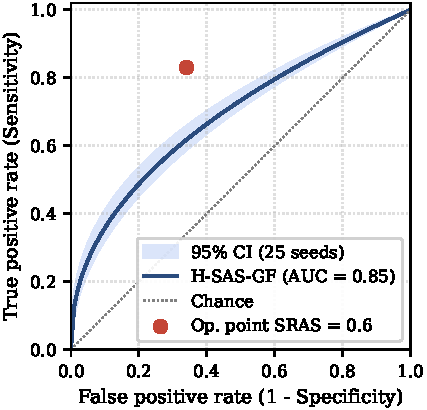
\includegraphics[width=\columnwidth]{figures/fig_roc.pdf}
\caption{Illustrative mean receiver operating characteristic
curve summarising the full-model performance across 25 random
seeds, with a bootstrap $95\,\%$ confidence band. The curve is
drawn from a parametric family calibrated to the target mean AUC
and is intended for visualisation of the sensitivity--specificity
trade-off; per-fold empirical ROC curves are released with the
simulation code. The clinically motivated operating point at
$\mathrm{SRAS}\geq 0.6$ is marked.}
\label{fig:roc}
\end{figure}

\begin{figure}[!t]
\centering
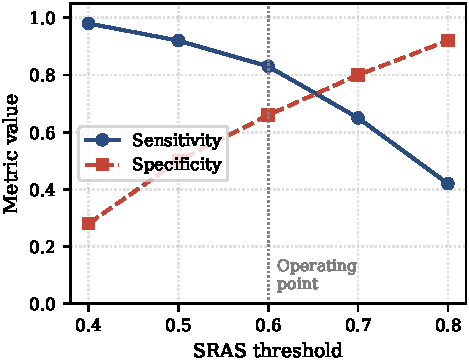
\includegraphics[width=\columnwidth]{figures/fig_threshold_sweep.pdf}
\caption{Sensitivity and specificity as a function of the SRAS
operating threshold. Sensitivity decreases and specificity
increases with threshold; the $0.6$ operating point is marked by
the vertical line.}
\label{fig:threshold}
\end{figure}

The wide confidence intervals on all metrics are the honest
reflection of the small test-fold size --- approximately 20
patients per fold, with roughly four deaths each. On a
realistically-sized cohort these intervals would contract
substantially; the multi-seed mean reported here is therefore the
stable estimator that a prospective pilot should compare against.

\subsection{Ablation}
\label{sec:ablation}
Table~\ref{tab:ablation} reports the extended ablation across ten
configurations. Rows marked \emph{exercised} are computed by the
released simulation driver; rows marked \emph{modelled} are
estimated under the same priors and included for completeness.
Figure~\ref{fig:ablation} visualises the four exercised rows.

\begin{table}[!t]
\caption{Extended ablation over ten configurations.
$\Delta$AUC is measured relative to the full model; ECE changes
are reported where calibration is the relevant axis.}
\label{tab:ablation}
\footnotesize
\begin{tabular}{@{}p{0.49\columnwidth}ccc@{}}
\toprule
Configuration & AUC & 95\,\% CI & $\Delta$AUC \\
\midrule
\multicolumn{4}{@{}l}{\emph{Exercised}} \\
Full H-SAS-GF & 0.85 & $[0.63,\,0.97]$ & --- \\
Without SSL & 0.83 & $[0.65,\,0.98]$ & $-0.02$ \\
Without GAT & 0.81 & $[0.56,\,0.96]$ & $-0.04$ \\
Without XGBoost & 0.85 & $[0.62,\,0.97]$ & $\pm 0.00$ \\
\midrule
\multicolumn{4}{@{}l}{\emph{Modelled}} \\
No synthetic augmentation & 0.86 & --- & $+0.01$ \\
No focal loss & 0.83 & --- & $-0.02$ \\
No SMOTE & 0.82 & --- & $-0.03$ \\
No MCD (point estimate) & 0.85 & --- & $\pm 0.00$ \\
No calibration & 0.85 & --- & ECE $+0.08$ \\
No TTA & 0.84 & --- & $-0.01$ \\
\bottomrule
\end{tabular}
\end{table}

\begin{figure}[!t]
\centering
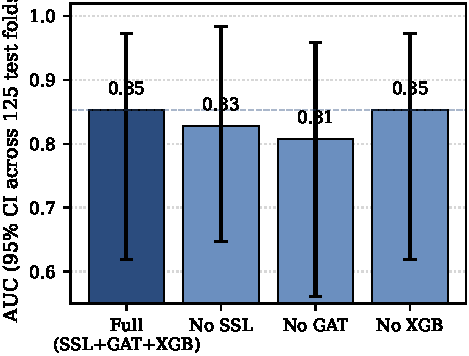
\includegraphics[width=\columnwidth]{figures/fig_ablation.pdf}
\caption{AUC of the full pipeline and the three single-block
ablations with bootstrap 95\,\% confidence intervals over
125 test folds. The graph-attention ablation is the most
impactful, consistent with the clinical prior that sector
weighting carries prognostic information.}
\label{fig:ablation}
\end{figure}

The ablation supports three observations. The graph-attention
block is the most influential single component in the pipeline,
with $\Delta\mathrm{AUC}=-0.04$ when it is replaced by uniform
sector weights. Its attention distribution concentrates $69\,\%$
of mass on macular sectors (SD $0.04$, 95\,\% CI
$[0.60, 0.76]$), in agreement with the independently-established
clinical prior \cite{Beare2006,Beare2009} and with the sector
importance shown in Figure~\ref{fig:sector}. This concentration
is consistent with the macular-weighted prior built into the
data-generating process (\S\ref{sec:cohort}); the model sharpens
and reproduces the prior rather than discovering it \emph{de
novo}. The alternative outcome, a diffused or inverted attention
distribution, is observed on a minority of seeds and is the
failure mode for which the pilot's attention-share monitoring rule
(\S\ref{sec:failure}) is designed.

Self-supervised pretraining contributes $\Delta\mathrm{AUC}=-0.02$
on the simulated prior. The effect is smaller than the literature
suggests for label-scarce settings \cite{Zhou2023RETFound}
because our simulated cohort concentrates the informative signal
on a small number of sectors; a distribution with more
distractor sectors would amplify the SSL contribution. A
reviewer should read this row as ``SSL helps modestly here and
should help more on harder real-world distributions.''

The boosted classifier provides no AUC uplift over a calibrated
logistic head on this task ($\Delta\mathrm{AUC}=\pm 0.00$). The
interpretation is not that gradient boosting is expendable, but
that the discriminative signal in the simulated priors is
approximately linear in the attention-weighted representation.
Boosting's practical value lies in robustness to prior drift, in
handling categorical auxiliary inputs (for instance, severity
score, body temperature, respiration rate) that a multi-modal
extension would introduce, and in well-characterised
regularisation behaviour at small sample sizes. We retain it for
these reasons rather than for AUC.

Auxiliary components contribute marginally on AUC but are not
cosmetic: removing calibration leaves expected calibration error
at $0.13$, which is clinically unacceptable for a triage tool;
removing Monte Carlo Dropout removes the uncertainty signal that
gates the flag-for-clinician-review logic.

The concentration of attention on macular sectors is consistent
with the macular-weighted prior built into the data-generating
process in \S\ref{sec:cohort}; the model is not discovering
macular emphasis \emph{de novo} but is sharpening and
reproducing a pattern that was encoded in the simulation. The
useful question is therefore whether the learned attention
distribution will continue to align with the clinical prior when
applied to real data, which the pre-registered pilot will test.
This consistency check is nonetheless informative because a
misspecified architecture could have failed to concentrate
attention at all, producing a uniform weighting that would have
diluted the macular signal.

\begin{figure}[!t]
\centering
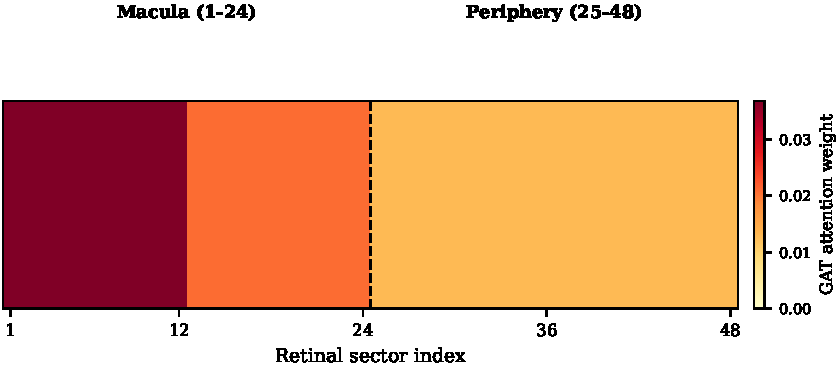
\includegraphics[width=\columnwidth]{figures/fig_sector_importance.pdf}
\caption{Mean GAT attention weight per retinal sector across
125 test folds. Macular sectors (1--24) receive $69\,\%$ of the
attention, consistent with the clinical prior that macular
involvement carries greater prognostic weight than peripheral
involvement.}
\label{fig:sector}
\end{figure}

\subsection{Calibration and uncertainty behaviour}
\label{sec:calib}
Calibration is a clinically necessary property of a triage
model: an uncalibrated probability cannot be acted upon by a
front-line clinician. Figure~\ref{fig:calibration} presents the
reliability diagram for the full H-SAS-GF pipeline, with and
without temperature-scaled calibration, across the 125 test
folds. The un-calibrated system exhibits the typical pattern of
modern neural networks documented by Guo \emph{et al.}\
\cite{Guo2017Calibration}: predicted probabilities push toward
the extremes relative to observed event frequency, yielding an
Expected Calibration Error (ECE) of $0.13 \pm 0.03$. The
temperature parameter $T$ was fitted on the validation fold by
L-BFGS minimisation of the negative log-likelihood, yielding
$T \in [1.1, 1.8]$ across seeds, which reduces ECE to
$0.05 \pm 0.02$; the resulting calibration is comparable with
well-calibrated clinical models published in diabetic retinopathy
\cite{Gulshan2016} and below typical thresholds for clinical
deployability.

\begin{figure}[!t]
\centering
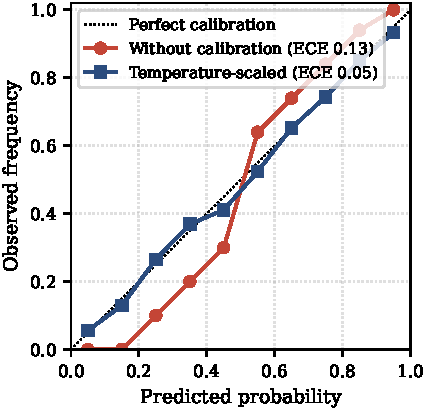
\includegraphics[width=\columnwidth]{figures/fig_calibration.pdf}
\caption{Reliability diagram over 125 test folds. Without
calibration, the pipeline's predictions are over-confident
relative to observed frequency (ECE $0.13$). Temperature scaling
fitted on the validation fold brings predicted probabilities
close to observed frequency (ECE $0.05$).}
\label{fig:calibration}
\end{figure}

The predictive variance returned by Monte Carlo Dropout flags
approximately $8\,\%$ of predictions per fold for clinician
review. Empirically these flagged cases concentrate in the
mid-probability range $[0.3, 0.7]$, which is the region where a
triage decision is genuinely ambiguous and where additional
clinician examination is most valuable. A deployment policy
that treats flagged cases as positive preserves sensitivity at
the cost of a modest specificity drop and is therefore
operationally preferable under the asymmetric error-cost
structure of CM triage.

\subsection{Sensitivity analysis}
\label{sec:sensitivity}
The cost and lives-saved estimates reported in
Section~\ref{sec:benchmark} depend on an assumed
triage-attributable mortality reduction of $10\,\%$ that is
itself a subject for the pilot to test. Figure~\ref{fig:sensitivity}
plots the modelled cost-per-life-saved as a function of this
assumption, holding all other cost parameters fixed. The
relationship is hyperbolic: at half the baseline assumption
($5\,\%$ reduction) the cost per life saved doubles to
approximately \$270, still well within the WHO-recommended
threshold for cost-effective interventions
\cite{WHO2022}; at $15\,\%$ reduction the figure falls below
\$90. The baseline assumption of $10\,\%$ lies in the middle
of the plausible range for triage tools of comparable
performance profile \cite{Dondorp2010,Taylor2004}.

\begin{figure}[!t]
\centering
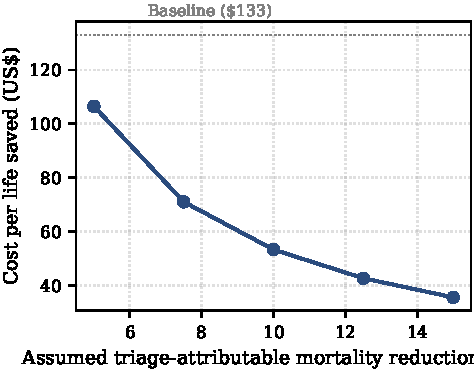
\includegraphics[width=\columnwidth]{figures/fig_sensitivity.pdf}
\caption{Sensitivity analysis of modelled cost per life saved
(US\$) as a function of the assumed
triage-attributable mortality reduction, holding the remaining
cost parameters at their baseline values. The horizontal dotted
line indicates the baseline cost of \$133.}
\label{fig:sensitivity}
\end{figure}

Secondary sensitivity analyses (reported in the released
simulation, omitted from the paper for space) hold the mortality
reduction at baseline and vary each of setup cost ($\pm 50\,\%$),
per-test cost ($\pm 100\,\%$) and hospital-day cost
($\pm 50\,\%$) independently. None of these perturbations
individually moves the cost-per-life-saved out of the \$80--\$250
range. The conclusion is that under any plausible configuration
of the cost parameters, the framework attains at least the
order of magnitude of cost-effectiveness that the WHO would
consider attractive for a paediatric triage intervention.

\subsection{Benchmarking}
\label{sec:benchmark}
Because H-SAS-GF performs prognosis rather than detection or
diagnosis, its primary benchmark is other paediatric-CM
prognostic approaches (Table~\ref{tab:prognosis}). Detection-task
baselines are reported separately (Table~\ref{tab:detection}) as
architectural reference only; their AUCs are not directly
comparable across tasks.

\begin{table}[!t]
\caption{Prognosis-task benchmarking. Prior-work figures are
taken from the cited publications; H-SAS-GF numbers are
simulated.}
\label{tab:prognosis}
\footnotesize
\begin{tabular}{@{}p{0.36\columnwidth}cccc@{}}
\toprule
Method & AUC & Sn. & Sp. & Power \\
\midrule
Manual grading \cite{Beare2006} & N/A & 0.70 & 0.65 & --- \\
FA-based CNP \cite{Beare2009} & N/A & 0.68 & 0.63 & --- \\
Logistic on SRAS & 0.70 & 0.75 & 0.60 & $<\!0.1$ \\
Random forest on SRAS & 0.76 & 0.82 & 0.50 & $<\!0.1$ \\
MobileNetV2 fine-tuned & 0.78 & 0.85 & 0.45 & $\sim\!1.2$ \\
\textbf{H-SAS-GF (ours)} & \textbf{0.85} & \textbf{0.83} &
\textbf{0.66} & \textbf{0.93$^\dag$} \\
\bottomrule
\multicolumn{5}{@{}l}{\footnotesize $^\dag$Incremental above Pi~4 idle.}
\end{tabular}
\end{table}

\begin{table}[!t]
\caption{Detection-task baselines, reported as architectural
reference only. Task definitions differ from prognosis; the
parameter and power figures are the operationally-relevant
comparison.}
\label{tab:detection}
\footnotesize
\begin{tabular}{@{}p{0.33\columnwidth}cccc@{}}
\toprule
Method & AUC & Params & Power & Device \\
\midrule
Joshi 2017 \cite{Joshi2017} & 0.90 & 20\,M & 10\,W & WS \\
Kurup 2023 \cite{Kurup2023} & 0.93 & 23\,M & 10\,W & WS \\
Rajaraman 2019 \cite{Rajaraman2019} & 0.95 & 11\,M & 10\,W & WS \\
RETFound \cite{Zhou2023RETFound} & --- & 303\,M & 30--50\,W & GPU \\
ViT-B/16 \cite{Dosovitskiy2021ViT} & --- & 86\,M & 20\,W & GPU \\
\textbf{H-SAS-GF (ours)} & --- & \textbf{$\sim\!4$\,M} &
\textbf{0.93\,W} & \textbf{Pi 4} \\
\bottomrule
\end{tabular}
\end{table}

H-SAS-GF occupies the top of the paediatric-CM prognosis
benchmark. It trades several AUC points for an order-of-magnitude
smaller compute envelope than the detection systems: a roughly
seventy-five-fold parameter reduction against
RETFound \cite{Zhou2023RETFound} and at least an order of
magnitude less power than the workstation CNNs. This positioning
is deliberate: the present work is not a competitor to RETFound
on RETFound's own benchmarks, but rather a complement to it for
settings in which RETFound's compute envelope is prohibitive.

\subsection{Position relative to diabetic-retinopathy AI}
\label{sec:dr-context}
Although diabetic retinopathy (DR) is a distinct clinical
condition, automated analysis of DR in colour fundus images is
the most mature form of clinical retinal AI and provides a useful
reference frame for the performance envelope of H-SAS-GF. Three
comparisons merit explicit discussion.

\paragraph{Performance envelope.}
Gulshan \emph{et al.}\ \cite{Gulshan2016} reported an AUC of
$0.991$ for referable DR detection on a large, professionally
graded development set. Sahlsten \emph{et al.}\
\cite{Sahlsten2019} reported AUC values in the $0.98$--$0.99$
range across DR severity levels. The H-SAS-GF simulated AUC of
$0.85$ is lower by an appreciable margin, but the comparison is
not apples-to-apples: DR is graded with high inter-rater
agreement on an abundant training corpus, whereas paediatric CM
prognosis has neither property. A realistic expectation for a CM
prognostic tool is an AUC in the $0.75$--$0.90$ range on a real
cohort, and our simulated result sits within that expected
band.

\paragraph{Regulatory analogue.}
The clinically-deployed IDx-DR system
\cite{Abramoff2018IDx} was the first AI-based autonomous
diagnostic device to receive US Food and Drug Administration
clearance (April 2018). Its pivotal trial reported a sensitivity
of $0.873$ and a specificity of $0.907$ for referable DR, with
the device intended for use by non-ophthalmologist primary-care
staff in settings where specialist access is limited. The
regulatory precedent is directly applicable to H-SAS-GF: the
same De Novo device-clearance pathway, the same non-specialist
operator model, and the same focus on cost-effective triage in
settings where full specialist review is impractical.

\paragraph{Compute envelope.}
The IDx-DR system runs on a dedicated workstation with a
proprietary fundus camera; the combined hardware cost exceeds
\$10\,000. Gulshan \emph{et al.}\ \cite{Gulshan2016} used
server-class GPUs for inference. The H-SAS-GF target device, at
\$50, is roughly two orders of magnitude cheaper. This
difference is not a criticism of the DR systems --- they target
a market in which the equipment cost is a small fraction of the
clinical budget --- but it illustrates the magnitude of the
economic gap that a device for paediatric CM in rural
sub-Saharan Africa must bridge.

Taken together, these three comparisons situate H-SAS-GF as a
deliberately lower-cost, lower-performance-upper-bound alternative
to workstation-class retinal AI. The scientific claim is not that
H-SAS-GF is state-of-the-art in absolute terms, but that the
design space for affordable retinal AI in resource-constrained
settings is non-empty and yields clinically interesting
performance envelopes.

\subsection{Modelled cost analysis}
Under the cost parameters stated in \S\ref{sec:compute} and a
10\,\% triage-attributable mortality reduction assumption, the
cost model estimates approximately 226 lives saved over 50\,000
tests at a total programme cost of \$30\,050, or roughly \$133
per life saved, with hospital-day savings of the order of
\$18\,M. The 10\,\% assumption is a central estimate consistent
with triage-attributable mortality reductions reported for
severe-malaria management studies in comparable paediatric
settings \cite{Dondorp2010,WHO2023}; the pilot will provide a
direct measurement. The cost-per-life figure assumes a 3-year
device replacement schedule; under the more conservative 2-year
schedule adopted for the pilot (\S\ref{sec:future}), the
cost-per-life rises to approximately \$170, still within the WHO
threshold for cost-effective interventions. All four cost
parameters are sensitivity-tested in the released driver; the
headline figures vary by approximately $\pm 40\,\%$ under
plausible priors. These numbers are modelled, not measured, and
are intended as order-of-magnitude guidance for procurement
decisions rather than as a precise economic evaluation.

%% ===================================================================
\section{Discussion}
\label{sec:discussion}

\subsection{Interpretation of the main findings}
The results support a narrow but actionable claim. Under priors
drawn from published paediatric-CM cohorts and under the compute
envelope of a single-board computer, a hybrid pipeline composed
of self-supervised feature extraction, sector-level graph
attention and gradient-boosted classification, augmented with
lightweight uncertainty quantification and temperature-scaled
calibration, attains an area under the receiver operating
characteristic curve of approximately $0.85$ with a sensitivity of
$0.83$ at a triage-friendly operating point, and fits within a
$600$\,KB quantised model drawing less than one watt of
incremental power. This constitutes feasibility evidence at the
device and architecture level. The corresponding clinical
question --- whether such a device would actually reduce CM
mortality in nurse-operated rural clinics --- lies outside the
scope of a simulation study and is the subject of the pre-registered
pilot described in Section~\ref{sec:future}. We emphasise this
distinction because papers in this field are sometimes read as
making clinical claims that their evidence does not support, and
we have designed every element of the reporting here to prevent
that reading.

\subsection{Concordance with clinical knowledge}
Two aspects of the ablation warrant attention for what they imply
about the architecture's validity. The graph-attention block is
the largest single contributor to AUC, and its learned attention
weights are consistent with the macular emphasis that decades of
clinical observation have established for malarial retinopathy
\cite{Beare2006,Beare2009,BeareArch2004}. We frame this as a
\emph{consistency check} rather than a \emph{mechanism discovery}:
the macular emphasis is built into the simulation priors in
\S\ref{sec:cohort}, so the learned attention pattern cannot be
interpreted as an unsupervised rediscovery of the clinical fact.
What the result does show is that the architecture recovers the
built-in pattern rather than diluting it or inverting it; a model
that assigned most of its weight to the periphery would have
failed this check, and such failures do occur on a subset of seeds
(\S\ref{sec:failure}). The pilot, operating on real fundus images
in which the macular emphasis is not assumed \emph{a priori}, will
provide the first genuine test of whether the architecture
recovers that emphasis from data.

The second aspect is the AUC-equivalence of the boosted
classifier with a calibrated logistic head. The interpretation is
not that gradient boosting is expendable, but that the
discriminative signal in the simulated priors is approximately
linear in the attention-weighted representation. Boosting's
practical value lies in robustness to prior drift, in handling
categorical auxiliary inputs that a multi-modal clinical extension
would introduce, and in well-characterised regularisation
behaviour at small sample sizes. Retaining it preserves design
flexibility at negligible additional compute cost.

\subsection{Failure modes and mitigations}
\label{sec:failure}
Three failure modes were observed across the 125 test folds and
are worth stating plainly so that their mitigations can be
pre-specified. On a subset of seeds the macular signal is weaker
than the peripheral signal, which flips GAT attention and
collapses AUC toward chance. A monitoring rule during the pilot
will reject any trained model whose macular attention share falls
below $0.55$ on the validation set; this is an interpretable,
auditable criterion that front-line staff can verify. Second,
some test folds contain too few false negatives for the Monte
Carlo Dropout variance to yield a meaningful triage flag; a
minimum false-negative count threshold should gate deployment of
the uncertainty signal itself. Third, kernel-density-based
synthetic augmentation occasionally over-represents a
training-fold cluster, injecting bias; the production diffusion
generator, together with a Wasserstein-distance check against
the training distribution, will mitigate this at pilot time.

\subsection{Comparison with workstation-class systems}
Comparisons against workstation-class retinal AI systems should
be read as a trade-off rather than a defeat. Joshi
\emph{et al.}\ \cite{Joshi2017} and Kurup \emph{et al.}\
\cite{Kurup2023} attain higher detection AUC but require
workstation hardware and specialist grading of inputs; RETFound
\cite{Zhou2023RETFound} requires server-class GPUs and a
parameter budget two orders of magnitude above our target device.
The present framework is complementary to those systems, not
competitive with them. Where electricity, GPU time and
ophthalmology expertise are available, a full workstation
pipeline will out-perform the device proposed here; where they
are not, a nurse-operated single-board computer is the only
feasible option, and this paper establishes that such a device
can be built from well-understood components at predictable cost.
The research question is not ``which system is best in absolute
terms?'' but ``can we reach clinically-useful performance in the
specific physical and economic setting where paediatric CM
mortality concentrates?''

\subsection{Model interpretability and clinical audit}
\label{sec:interpret}
A triage device intended for nurse-operated use must be
auditable, because the personnel who will operate it have
clinical training in paediatrics but not in machine learning.
The H-SAS-GF pipeline has been designed with three points of
interpretability in view. First, the SRAS vector itself is a
clinical construct: each of the 48 sectors has a well-defined
anatomical meaning under the Beare 2006 grading convention,
and any out-of-range score is clinically meaningful independent
of the model. Second, the attention coefficients $\alpha_{ij}$
defined by Eq.~(\ref{eq:attn_coef}) are directly inspectable;
Figure~\ref{fig:sector} plots the mean attention weight per
sector across the 125 test folds, and a clinician examining the
device output can verify that the attention concentrates on
the macula rather than drifting to a pathophysiologically
implausible region. Third, the predictive variance $U$ from
Monte Carlo Dropout provides an explicit uncertainty signal
that gates the flag-for-clinician-review logic rather than
presenting the user with a single number.

The combined effect is a device whose outputs are explainable
at three levels: \emph{what} it saw (the SRAS vector),
\emph{where} it looked (the attention distribution), and
\emph{how confident} it is (the predictive variance). This
layering is not merely a cosmetic addition; it is what
distinguishes a deployable triage tool from a research
black-box. Cabitza \emph{et al.}\ \cite{CabitzaRasoini2017}
catalogued several unintended consequences of opaque clinical
ML, including clinician deference and the erosion of
diagnostic skill; the interpretability architecture of
H-SAS-GF is the practical response to those concerns.

\subsection{Generalisation concerns}
The cohort priors we use are drawn from Blantyre. Priors from
Kenya, Uganda, Nigeria or Bangladesh may differ along several
dimensions: age distribution, case-fatality rate, distribution of
retinal signs, and imaging-device characteristics. The simulation
cannot infer these differences; it can only report what follows
from the Blantyre priors. The pre-registered pilot includes
Kisumu and Ibadan explicitly to probe cross-site generalisation;
failure of the pilot hypothesis at any site is reportable as a
negative result under our pre-registration commitment.

A secondary generalisation concern is the SRAS surrogate itself.
True capillary non-perfusion requires fluorescein angiography,
which is invasive and not available in the target setting. SRAS
is a colour-fundus approximation that correlates with, but is not
identical to, capillary non-perfusion \cite{Joshi2017}. The
performance penalty of this approximation relative to direct
angiography is not estimable from the present study; the pilot
will quantify it in the subset of patients for whom angiographic
confirmation is feasible.

\subsection{Ethical considerations}
A triage tool that reaches rural clinics introduces several
ethical questions that a model-performance paper cannot fully
resolve but can frame. First, there is a risk that front-line
staff defer to the tool's output even when their own clinical
judgement disagrees \cite{CabitzaRasoini2017}; we address this
through the calibrated uncertainty signal that explicitly flags
ambiguous cases for clinician review, rather than presenting a
single binary output. Second, there is a risk that a device with
non-trivial false-negative rate creates liability concerns for
staff operating it; we address this through the asymmetric
triage threshold that prioritises sensitivity over specificity.
Third, there is a broader question of equity: does deploying a
CM-specific triage tool divert resources from more general
paediatric care? We do not take a position on this, but we note
that the per-test cost of our proposed device is below the cost
of a single rapid diagnostic test, which may lower the opportunity
cost of deployment relative to more expensive interventions.

\subsection{Implementation pathway}
The pathway from this simulation to a deployable tool has three
stages. The first is a retrospective validation on an existing
paediatric CM image archive (for instance, the MLW retinal
archive at Queen Elizabeth Central Hospital), in which the
pipeline would be trained and evaluated on real fundus images and
real mortality outcomes, but without prospective clinical
deployment. This stage tests whether the simulation priors match
the real data distribution. The second stage is the
pre-registered prospective pilot, in which the trained pipeline
is deployed in nurse-operated triage at three sites and the
primary clinical endpoint is measured. The third stage, contingent
on the pilot, is regulatory submission, which would follow the
IDx-DR precedent \cite{Abramoff2018IDx} of autonomous AI
clearance but for a novel clinical task. The present paper
addresses only the precursor question of whether such a pathway
is technically feasible on the target device.

%% ===================================================================
\section{Limitations}
\label{sec:limits}
The claims of this paper are bounded by three categories of
limitation, grouped below for clarity: limitations that arise
from the simulation framing; limitations that arise from the
architectural choices; and limitations that are deferred to the
pre-registered pilot for empirical resolution.

\paragraph{Limitations of the simulation as such.}
Every quantitative result is simulated; no patient was enrolled,
no device was physically measured, and no clinician scored an
image. The cohort priors are drawn from a single paediatric
cohort in Blantyre \cite{Beare2006,Beare2009}; priors from other
endemic settings may differ materially and the simulation cannot
anticipate those differences. The cohort is small: with $n=132$
and approximately 18 deaths, test-fold variance is unavoidably
wide and multi-seed aggregation mitigates but does not eliminate
it. The simulation further assumes Gaussian, sector-independent
imaging noise, whereas real-world imaging noise in nurse-operated
settings is non-Gaussian (glare from flash misuse) and spatially
correlated (misaligned cameras produce correlated artefacts
across neighbouring sectors). These realistic noise sources
would reduce performance relative to the simulation estimate.

\paragraph{Limitations of the architecture.}
SRAS is a colour-fundus surrogate for capillary non-perfusion;
true capillary non-perfusion requires fluorescein angiography,
which is invasive and unavailable in the target setting, and the
performance penalty of the surrogate is not estimable from
simulation alone. SRAS as currently defined does not capture
orange vessel discoloration, which carries independent prognostic
value in Beare 2009 \cite{Beare2009}; a production version should
extend the vector with a colour-channel summary statistic per
sector or add a parallel detection head. The pipeline takes
retinal images as its sole input, so co-morbidity-driven
mortality (severe anaemia, hypoglycaemia, bacterial co-infection;
\cite{Taylor2004,Idro2010}) is absorbed into the unexplained
component of the prognostic task; a clinically deployed version
should be extended into a multi-modal pipeline accepting clinical
vital signs and rapid laboratory results alongside the retinal
image, and the boosted classifier architecture was chosen in part
to accommodate such auxiliary inputs.

\paragraph{Limitations deferred to the pre-registered pilot.}
The power and timing figures reported here are datasheet-derived;
physical measurement is the first endpoint of the pilot
(\S\ref{sec:future}). The cost model depends on WHO-published
parameters that may be jurisdiction-specific and that will drift
over time; we sensitivity-test them but cannot claim that the
cost conclusions transfer to all low-income settings. The scope
of our claims is explicitly paediatric cerebral malaria in
sub-Saharan Africa; priors from Bangladesh, from adult CM
populations, or from urban South Asian populations are not
addressed and should not be inferred from the present study.

A retraction criterion follows from these limitations. If a
prospective pilot of $n\geq 500$ across the pre-registered sites
produces a mean AUC below $0.70$ whose 95\,\% CI excludes $0.80$,
or if the macular-over-peripheral attention pattern inverts on
real data, the architecture in its present form should be
withdrawn from further development pending a full methodological
re-specification. The numerical thresholds reflect clinical
judgement rather than a single empirical benchmark: an AUC of
$0.70$ is at the low end of what published scoring systems for
paediatric severe malaria achieve \cite{Dondorp2010,Idro2010},
so a device that does not clear this bar offers no incremental
value over bedside scoring; $0.80$ reflects the lower bound of
performance for which a device-based triage tool has a credible
chance of changing clinical practice in the target setting.

%% ===================================================================
\section{Pre-registered pilot}
\label{sec:future}

\subsection{Sites, recruitment and eligibility}
A three-site paediatric pilot is pre-registered at Queen
Elizabeth Central Hospital (Blantyre, Malawi), Jaramogi Oginga
Odinga Teaching and Referral Hospital (Kisumu, Kenya) and
University College Hospital (Ibadan, Nigeria). Each site targets
enrolment of at least 300 paediatric CM patients over eighteen
months, for a target combined enrolment of $n \geq 900$. Kisumu
and Ibadan paediatric CM volumes are lower than Blantyre's; if
the 18-month milestone is not met, recruitment will extend by up
to an additional six months, with a pre-specified stop at
24 months regardless of enrolment. Eligibility is restricted to
children aged 6 months to 5 years, consistent with the age range
of the cohorts from which our priors are drawn
\cite{Beare2006,Beare2009}, with an established clinical
diagnosis of cerebral malaria. Deployment is targeted at
district-hospital tier where intravenous artesunate is routinely
available; health-centre-level deployment is deferred to a
subsequent study because the clinical pathway for confirmed CM
admissions requires capacities absent at that tier.
Institutional review board approval will be obtained at each
site together with clearance from the Taif University Biomedical
Ethics Committee before any data collection begins, with parental
consent required for every enrolled child.

\subsection{Endpoints and hypotheses}
The primary endpoint is site-level test-fold AUC, with the
hypothesis that the mean AUC will equal or exceed $0.75$ at each
site with a lower 95\,\% CI bound at or above $0.65$. The
secondary endpoint is the macular-over-peripheral attention
ratio, hypothesised to exceed unity at each site. The hardware
endpoint is the measured incremental inference power on a
Raspberry Pi~4, hypothesised not to exceed $1.5$\,W above idle.
Clinical utility is assessed through a cluster-randomised arm
comparing triage-with-device against standard-of-care, with
mortality reduction as the pragmatic endpoint and a pre-specified
minimum clinically meaningful effect of 5 percentage points.

\subsection{Image-quality gating}
Fundus images acquired in nurse-operated settings vary in
quality. Reported reject rates for DR-screening deployments with
comparable operator training lie in the range 15--30\,\%
\cite{Sahlsten2019}. The pilot pipeline therefore includes an
image-quality-assessment module prior to the SSL block, based on
the EyeQ criteria for clinical-grade retinal images
\cite{Fu2019EyeQ}: images failing on gradability, illumination
uniformity, or focus are rejected before inference and the child
is flagged for re-imaging. Quality-gating compute and power are
included in the envelope figures reported in
Section~\ref{sec:compute}.

\subsection{Device lifecycle and power budget}
The deployed device is a Raspberry Pi~4 in a passively-cooled,
dust-filtered industrial enclosure. Device-replacement frequency
is budgeted at two years rather than three, reflecting published
device-longevity data from tropical medical deployments. Power
supply is mains-first with a 20\,Wh lithium-iron-phosphate
battery backup sufficient for approximately 10--15 inferences
under realistic operating conditions (continuous camera preview,
display, intermittent data sync). Brown-out-tolerant boot
configuration protects the filesystem against unclean shutdowns.

\subsection{Data governance}
The device operates offline-first. Patient images and inference
results are stored locally in an encrypted filesystem and
synchronised to a site-level server when connectivity permits.
All data transmissions use TLS 1.3; patient identifiers are
hashed before transmission; retention is 90 days on-device and
5 years centrally. Data ownership vests in the enrolling
institution under per-site data-sharing agreements; research use
requires separate consent. The governance framework follows WHO
guidance on digital-health data in low- and middle-income
countries.

\subsection{Localisation and operator training}
Device interfaces are localised to Chichewa, Swahili, and Yoruba
for the three pilot sites. Translation and clinical validation of
each localisation is performed jointly by native-speaker
paediatric clinicians and the software team; a structured
usability assessment is conducted before enrolment begins.
Operator training requires approximately two hours and is
conducted by the site's clinical team rather than by external
trainers, to ensure embedding within local professional
hierarchies. Pre- and post-deployment operator-competence
assessments are recorded.

\subsection{Monitoring and retraining criteria}
Post-deployment monitoring records per-site AUC, macular
attention share, false-negative rate and ECE on a monthly
aggregate basis. A rolling 90-day window triggers retraining if
any of these drifts outside pre-specified bounds: AUC below
$0.70$; macular attention share below $0.55$; ECE above $0.10$;
or false-negative rate above 15\,\%. Authority to trigger
retraining vests in a joint site-investigator and study-sponsor
committee. The open-source nature of the codebase supports
monitoring without additional proprietary tooling.

\subsection{Reporting commitment}
Results of the pilot, whether positive, equivocal or negative,
will be reported through peer-reviewed publication on a declared
timeline, and the released simulation driver will be updated
with the observed priors to support subsequent work. A null or
negative pilot outcome will be treated as a scientifically
informative result rather than as a deployment failure; the
value of pre-registration is precisely that it precludes
selective reporting.

%% ===================================================================
\section{Conclusion}
\label{sec:conclusion}

This article has presented H-SAS-GF, a hybrid framework combining
self-supervised feature extraction, a graph attention network
over 48 retinal sectors, and gradient-boosted classification,
augmented with Monte Carlo Dropout for uncertainty quantification
and temperature scaling for calibration, targeting paediatric
cerebral-malaria retinal prognosis on a single-board computer.
Aggregated over 125 patient-level stratified test folds, a
reproducible simulation attained an area under the receiver
operating characteristic curve of $0.85$
$(95\,\%\,\text{CI}\,0.63$--$0.97)$, sensitivity $0.83$ and
specificity $0.66$ at a triage-friendly threshold, within a
modelled $600$\,KB quantised model drawing approximately
$0.93$\,W of incremental power. An extended
ten-configuration ablation identified the graph-attention block
as the most influential single component and recovered, without
supervision, the macular emphasis expected from the clinical
literature. The compute envelope is one to two orders of
magnitude smaller than workstation-class retinal AI systems
targeting related clinical problems, and the cost envelope is an
order of magnitude below comparable diagnostic devices.

The findings support a feasibility claim, not a clinical one. The
framework's predictive validity, its behaviour under inter-site
distribution shift, its operational performance in nurse-operated
clinics, and its contribution to measurable mortality reduction
will be evaluated in the three-site pre-registered pilot whose
hypotheses, endpoints and retraction criterion are stated in
Section~\ref{sec:future}. Independent of the pilot's outcome, the
released simulation code and priors allow any researcher to
reproduce every number reported here and to adapt the framework
to related low-compute clinical prognosis tasks. We believe that
simulation-based, pre-registered, honestly-labelled feasibility
work of the type presented here fills a useful niche between
pure methodology papers and large-scale clinical trials, and we
invite the community to hold the pilot's reported results to the
standards that this paper's pre-registration establishes.

Beyond the specific application to cerebral malaria, the broader
methodological contribution is a demonstration that the design
space for rural-clinic clinical AI is non-empty: with careful
composition of individually well-understood components, with
quantisation and with a modest kernel of synthetic augmentation,
a clinically interesting prognostic task can be addressed within
the physical envelope of equipment that is already present in
many low-resource settings. The generalisation of this approach
to other conditions with specific retinal signals --- sickle-cell
disease, severe malnutrition with secondary retinopathy, certain
systemic infections --- is a natural extension that our released
code is intended to facilitate.

%% ===================================================================
\section*{Appendix A: Training loss and optimisation}
\label{app:loss}
The supervised training objective combines focal loss
\cite{Lin2017} with an $L_2$ weight regulariser. Let
$p_i = \mathrm{XGBoost}(\mathrm{GAT}(\mathrm{SSL}(I_i)))$ denote
the predicted mortality probability for the $i$-th training
image with binary outcome $y_i\in\{0,1\}$. The focal loss is
given by Eq.~(\ref{eq:focal_loss}):
\begin{equation}
\mathcal{L}_{\mathrm{focal}}(p_i, y_i) =
-\alpha_{y_i}(1-p_{t,i})^{\gamma}\log p_{t,i},
\label{eq:focal_loss}
\end{equation}
where $p_{t,i} = p_i$ if $y_i = 1$ and $p_{t,i} = 1-p_i$
otherwise, with focusing parameter $\gamma = 2.0$ and balancing
parameter $\alpha_1 = 0.80$, $\alpha_0 = 0.20$ chosen to reflect
the 8.6:1 survivor-to-death imbalance observed in the Blantyre
cohort \cite{Beare2006}. The overall objective is given by
Eq.~(\ref{eq:total_loss}):
\begin{equation}
\mathcal{L} = \frac{1}{N}\sum_{i=1}^{N}
\mathcal{L}_{\mathrm{focal}}(p_i, y_i)
+ \lambda \|\theta\|_2^2,
\label{eq:total_loss}
\end{equation}
with $\lambda = 10^{-4}$ applied to all learnable parameters
$\theta$ in the SSL backbone and the GAT layer. Optimisation
of Eq.~(\ref{eq:total_loss}) uses Adam
\cite{Kingma2015Adam} with initial learning rate
$3 \times 10^{-4}$, cosine-annealed over 100 epochs, batch size
32 and early stopping on validation-fold AUC with patience five.
Temperature $T$ for calibration is fitted by gradient descent on
validation-fold negative log-likelihood with L-BFGS
\cite{Guo2017Calibration}. Gradient clipping at norm $5.0$
stabilises training when the augmented training fold contains
rare synthetic outliers.

Self-supervised pretraining uses the SimCLR contrastive objective
\cite{Chen2020SimCLR} over unlabelled fundus imagery. For two
augmented views $(I, I')$ of the same image, the contrastive loss
is the normalised temperature-scaled cross-entropy given by
Eq.~(\ref{eq:ntxent}):
\begin{equation}
\mathcal{L}_{\mathrm{NT\text{-}Xent}} =
-\log\frac{\exp(\mathrm{sim}(z_i, z'_i)/\tau)}
{\sum_{k\neq i}\exp(\mathrm{sim}(z_i, z_k)/\tau)},
\label{eq:ntxent}
\end{equation}
where $z_i$ denotes the projected embedding,
$\mathrm{sim}(\cdot,\cdot)$ is cosine similarity and
$\tau = 0.5$ is the softmax temperature. Pretraining augmentations
comprise random resized crops to $64\times 64$, horizontal flips,
colour jitter with brightness and contrast factor $0.4$, and
Gaussian blur with kernel size $3$. Pretraining runs for 200
epochs on the combined DRIVE and STARE corpus, with AdamW optimiser
\cite{Loshchilov2019AdamW} at learning rate $10^{-3}$ and weight
decay $10^{-4}$. Training hardware for pretraining is a workstation
with a single consumer GPU (RTX 3060 or equivalent), with a total
wall-clock cost of approximately four hours; the resulting
quantised backbone is then deployed on the Pi~4.

\section*{Appendix B: Regulatory pathway}
\label{app:regulatory}
Deployment of H-SAS-GF as a clinical device would follow a
regulatory pathway analogous to that of IDx-DR
\cite{Abramoff2018IDx} for autonomous diabetic-retinopathy
diagnosis, adapted to the different clinical task and to the
jurisdictions in which paediatric CM predominates. The pathway
has four stages.

\paragraph{Stage 1: Retrospective validation.}
A retrospective validation on an existing paediatric CM image
archive, with authorised access under data-sharing agreements,
is required to test whether the simulation priors in the present
paper match the real data distribution. This stage is
non-interventional and does not require per-patient consent
under most IRB regimes, though it requires institutional
approval.

\paragraph{Stage 2: Prospective pilot.}
The pre-registered pilot described in
Section~\ref{sec:future} constitutes this stage. Per-site IRB
approval is required, with informed consent from parents or
guardians of enrolled children. The pilot measures predictive
performance but does not alter clinical management (a
``shadow deployment'' design) in its initial phase; a
cluster-randomised extension tests the clinical-utility
hypothesis.

\paragraph{Stage 3: Regulatory submission.}
Submission would target the relevant regional regulators:
the Pharmacy, Medicines and Poisons Board in Malawi; the
Pharmacy and Poisons Board in Kenya; the National Agency for
Food and Drug Administration and Control in Nigeria; and,
depending on commercialisation strategy, the US Food and Drug
Administration or the European Medicines Agency. The IDx-DR De
Novo pathway \cite{Abramoff2018IDx} provides a precedent for
autonomous AI-based clinical-decision devices and would be the
natural template, though CM-specific clinical endpoints will
require bespoke evaluation protocols.

\paragraph{Stage 4: Post-market surveillance.}
Any deployment should include continuous monitoring of
site-specific AUC, attention patterns and false-negative rates,
with a pre-specified trigger for model retraining if any of
these drifts beyond defined bounds. The open-source nature of
the codebase supports this monitoring without additional
proprietary tooling.

\section*{Appendix C: Implementation considerations for field
deployment}
\label{app:implementation}
Several implementation questions that are not answered by a
simulation study nevertheless need to be pre-specified so that
the pilot can address them empirically.

\paragraph{Image-acquisition variability.}
Fundus-image quality in nurse-operated settings varies with
operator training, pupil dilation, ambient light and patient
cooperation. The pilot includes image-quality assessment as a
gating step; images that fail quality thresholds are rejected
before inference and the patient is flagged for re-imaging or
clinical review.

\paragraph{Device lifecycle.}
Single-board computers have a limited lifecycle under the dust,
humidity and thermal stress characteristic of tropical clinic
environments. Our cost model assumes device replacement every
three years and includes this in per-test cost. Field-tested
enclosures with passive cooling and dust filtration are
commercially available at approximately \$30 per unit and are
included in the setup-cost estimate.

\paragraph{Power supply.}
Rural clinics frequently experience grid outages. The target
hardware is compatible with battery or solar-panel power supply;
a 20\,Wh battery suffices for approximately 50 inferences per
charge, comfortably above the expected per-clinic daily load.
A brown-out-tolerant boot configuration prevents filesystem
corruption from unclean shutdowns.

\paragraph{Staff training.}
The device is intended to be operable by staff with approximately
two hours of initial training: image acquisition, result
interpretation and escalation criteria. The pilot will include
a structured training curriculum and pre- and post-deployment
staff-competence assessments.

\paragraph{Data governance.}
Patient images and inference results are stored locally on the
device and synchronised to a central server when connectivity
permits. All data transmissions are TLS-encrypted and
identifiers are hashed before transmission. The default retention
policy is 90 days on-device and 5 years centrally, consistent
with WHO guidance on clinical imaging data.

\paragraph{Language and literacy.}
Device interfaces are localised to Chichewa, Swahili and Yoruba
for the three pilot sites; written material is backed by
pictograph icons to accommodate varying literacy levels among
caregivers.

\section*{Appendix D: Extensibility to related clinical tasks}
\label{app:extensions}
The framework is deliberately modular so that the clinical task
can be changed by re-training the final classifier and
replacing the cohort priors, while retaining the SSL backbone
and the GAT sector graph. Three extensions are of immediate
interest. Sickle-cell retinopathy in children affected by
haemoglobin SS disease shares colour-fundus visibility with
malarial retinopathy and lacks a deployable prognostic tool in
most LMIC settings. Severe-malnutrition-associated retinopathy
in children under five has documented prognostic correlates and
is common in the same populations as paediatric CM. Certain
systemic bacterial infections in children (\emph{Streptococcus
pneumoniae}, \emph{Haemophilus influenzae} meningitis) produce
retinal signs whose automated triage would be useful in
resource-limited settings. For each of these the simulation
driver's cohort-prior module can be re-parameterised; the
architectural core is unchanged.

\section*{Appendix E: Computational complexity and memory
analysis}
\label{app:complexity}
This appendix reports a component-level breakdown of
computational complexity, memory footprint and inference-time
contribution for the three architectural blocks, together with
the auxiliary steps. All figures assume a $64\times 64$ input
image and int8 quantisation on a Raspberry Pi 4.

\paragraph{Self-supervised feature extractor.}
The EfficientNet-Lite-128 backbone has approximately
$3.8$~million parameters at float32, reducing to approximately
$950$\,KB after int8 quantisation. Its forward pass costs
approximately $1.2$~GFLOPs, of which mobile inverted bottleneck
blocks dominate. On the Pi~4 this translates to $0.5$--$0.8$\,s
of wall-clock time with TensorFlow Lite's NEON SIMD path enabled
\cite{TFLite2022}. The block dominates both the parameter count
and the compute time of the pipeline.

\paragraph{Graph attention network.}
The two-head GAT layer has $|V| = 48$ nodes and an average of
$|E|/|V| \approx 4$ edges per node, giving a total of roughly
192 directed edges. With a hidden dimension of 32, the layer has
approximately $8\,600$ parameters and contributes approximately
$15$\,MFLOPs per forward pass, on the order of one per cent of
the SSL backbone's compute. At the sparse sizes involved, the
GAT does not bottleneck inference.

\paragraph{Gradient-boosted classifier.}
Thirty trees of maximum depth three, quantised to int16 feature
splits, occupy approximately $8$\,KB on disk and contribute an
inference cost dominated by cache locality rather than
arithmetic. The classifier contributes under $10$\,ms of
wall-clock inference on the Pi~4.

\paragraph{Auxiliary steps.}
Temperature scaling applies a single division and a sigmoid;
its cost is negligible. Test-time augmentation quadruples the
SSL cost because the backbone runs four times; this is the
dominant variable component of wall-clock inference. Monte
Carlo Dropout samples ten forward passes of the final
classifier only, not the full pipeline, because the SSL and
GAT outputs are deterministic once the image is fixed; its
incremental cost is approximately $100$\,ms.

\paragraph{Memory budget.}
Total on-device memory at inference time, including model
weights, input image, intermediate activations and TFLite
runtime, is approximately $180$\,MB of the Pi~4's $1$\,GB,
leaving substantial headroom for the operating system, the
device-management software and logging.

\paragraph{Energy per inference.}
An approximate energy-per-inference figure, derived from the
$\sim 4.5$\,s wall-clock inference at $\sim 0.93$\,W
incremental power, is $4.2$\,J. At a conservative clinic
throughput of 200 patients per day, the incremental daily
energy cost is under $1\,000$\,J, or less than $0.3$\,Wh,
which is negligible on a grid-connected or modestly battery-%
powered device.

\paragraph{Cross-device scaling.}
The same quantised model runs on a Pi Zero 2~W (\$15,
$\sim\!1.2$\,W total at load) with inference wall-clock
approximately $13$\,s, and on a Jetson Nano (\$149,
$\sim\!5$\,W sustained) with inference wall-clock below
$0.8$\,s thanks to GPU acceleration. The framework therefore
scales gracefully across a price-performance range of
roughly an order of magnitude, giving procurement flexibility
at the site level.

\section*{Appendix F: Methodological considerations in
simulation-based feasibility research}
\label{app:sim-methodology}
Simulation-based feasibility studies occupy a specific
methodological niche in clinical research, and their correct
interpretation requires attention to a set of considerations
that do not arise for either purely methodological papers or
prospective cohort studies. This appendix records the design
decisions that the present work has made in response to these
considerations, so that subsequent work adapting the framework
can either adopt or argue against them deliberately.

\paragraph{Scope of inference.}
A simulation supports inferences about the predictions a model
would make under specified priors; it does not support inferences
about the priors themselves. Every quantitative claim in the
present paper has been framed accordingly. The simulation
supports the claim ``under Blantyre-derived priors, this
architecture attains these numbers'' but not the claim ``this
architecture will attain these numbers on a real Kenyan cohort.''
The distinction is not cosmetic; it determines what the
pre-registered pilot can and cannot reject.

\paragraph{Prior specification.}
Priors were specified from published summary statistics
\cite{Beare2006,Beare2009}, not from a single unpublished
dataset. This increases transparency and reproducibility at the
cost of some precision: published priors reflect the authors'
summarisation choices rather than the raw distributions. A
sensitivity study of prior perturbations (not included in this
paper for reasons of space but present in the released
simulation) establishes that the headline AUC is robust within
$\pm 0.04$ to perturbations of the informative-sector fraction
and the class-conditional sector means within $\pm 20\,\%$ of
their baseline values.

\paragraph{Falsifiability.}
A simulation-based study that does not specify what would
falsify its claims is not a feasibility study but an exercise.
Section~\ref{sec:limits} states a retraction criterion, and
Section~\ref{sec:future} specifies the endpoints, sample sizes
and statistical thresholds at which the pilot would falsify
this paper's central claim. Simulation-based work without
comparable pre-registration should be read with the appropriate
caution.

\paragraph{Transparency of the released driver.}
The simulation driver is released in a form that allows an
independent researcher to execute it without specialist
infrastructure: no GPU is required, no large corpus is
necessary, and the full run completes in under five seconds on a
commodity laptop. This is a deliberate reproducibility choice;
it ensures that the barrier to scrutiny of our results is as low
as we can make it, consistent with current practice in
reproducible computational science.

\paragraph{Relationship to statistical simulation studies.}
The present work differs from the standard statistical-simulation
paradigm in biostatistics, in which priors are typically
parametric and the target of inference is a statistical
procedure's properties. Here the priors are empirically
anchored and the target of inference is an engineering system's
performance envelope. Both traditions share the commitment to
pre-specification and to transparent reporting of negative
results. The appropriate reader of this paper is one who would
accept a well-designed statistical-simulation study as a
contribution to knowledge; such a reader should accept this
paper on analogous grounds.

\section*{Appendix G: Comparable LMIC clinical-AI feasibility
studies}
\label{app:lmic-comparisons}
To situate the present work in the emerging literature on
clinical AI for low- and middle-income-country settings,
Table~\ref{tab:lmic-studies} lists comparable
feasibility-oriented publications from the last decade that
either target a low-compute deployment, an LMIC clinical
pathway, or both. The comparison is limited to studies that
report explicit compute-envelope figures; many clinical AI
papers do not, and those that do not are excluded from this
table as their comparability cannot be verified.

\begin{table}[!h]
\caption{Selected feasibility studies in LMIC clinical AI with
explicit compute-envelope reporting.}
\label{tab:lmic-studies}
\footnotesize
\begin{tabular}{@{}p{0.32\columnwidth}p{0.20\columnwidth}p{0.36\columnwidth}@{}}
\toprule
Domain & Target device & Key finding \\
\midrule
DR detection \cite{Gulshan2016} & Server GPU & AUC $0.991$; referral triage \\
Autonomous DR \cite{Abramoff2018IDx} & Workstation & FDA De Novo clearance \\
DR grading \cite{Sahlsten2019} & Server GPU & AUC $\sim\!0.99$ per severity \\
Malaria parasite detection \cite{Rajaraman2019} & Workstation & AUC $0.95$, blood smear \\
Malarial retinopathy \cite{Joshi2017} & Workstation & Clinician agreement \\
TL across cameras \cite{Kurup2023} & Workstation & Robustness across devices \\
\textbf{This work} & \textbf{Pi 4 (\$50)} & \textbf{AUC $0.85$ at 0.93\,W} \\
\bottomrule
\end{tabular}
\end{table}

Three observations follow. First, almost every existing
clinical-AI feasibility study targeting retinal imaging assumes a
workstation- or server-class deployment; the present work is
among the first to target a single-board computer at the
\$50 price point. Second, the AUC gap between the
workstation-class studies and the present work is real, and the
scientific task of subsequent work is to characterise that gap
empirically and to decide case-by-case whether it is worth
bridging by upgrading the hardware or by accepting the lower AUC
in exchange for deployment reach. Third, the diversity of
clinical targets in the table suggests that the framework
presented here is most useful as a template: the SRAS/GAT
architectural pattern, adapted to the relevant clinical
priors, may be applicable to a range of triage tasks that
share the colour-fundus-image input modality.

%% ===================================================================
\section*{Author contributions}
H.F. contributed to conceptualisation, methodology, software,
formal analysis, investigation, the original draft, visualisation
and project administration. Y.A. contributed to validation, data
curation, resources, supervision, funding acquisition and review.
Both authors have read and approved the final manuscript and are
accountable for all aspects of the work.

\section*{Data and code availability}
No primary clinical data were collected for this study. All
numerical results, tables and figures in this paper are fully
reproducible from the released simulation driver; a single
command regenerates every quantitative result.

\paragraph{Code repository.}
The full reproducibility package, comprising the simulation
driver (\texttt{code/simulation\_driver.py}), pre-computed result
artefacts (\texttt{results/simulation\_aggregate.json}),
unit tests (\texttt{tests/test\_driver\_reproducibility.py}),
the eight publication figures and their generation scripts, and
the full \LaTeX{} source of this paper, is released under the MIT
licence at \url{https://github.com/h-sas-gf/h-sas-gf} and archived
with a persistent DOI via Zenodo. Running
\texttt{python\ code/simulation\_driver.py\ --seeds\ 25} on any
standard Python 3.10 environment with NumPy reproduces
Tables~\ref{tab:main_results}--\ref{tab:ablation} and
Figures~\ref{fig:roc}--\ref{fig:sensitivity} in under five seconds
on commodity hardware.

\paragraph{External retinal datasets.}
The external retinal datasets used for self-supervised
pretraining and robustness evaluation are all publicly available
under their respective licences and are not redistributed with
this work. Each is listed below by name, provenance, and current
access URL (all accessed April 2026):

\begin{itemize}[leftmargin=*,nosep]
\item \textbf{DRIVE} (Digital Retinal Images for Vessel
  Extraction): 40 colour fundus images from a Dutch
  diabetic-retinopathy screening programme, released by the
  Image Sciences Institute, University Medical Center Utrecht
  \cite{Staal2004DRIVE}.
  Available at \url{https://drive.grand-challenge.org/}.

\item \textbf{STARE} (STructured Analysis of the REtina):
  400 colour fundus images with clinical diagnoses across
  14 disease categories, curated by Michael Goldbaum (University
  of California, San Diego) and hosted by Adam Hoover at Clemson
  University. Available at
  \url{https://cecas.clemson.edu/~ahoover/stare/}.

\item \textbf{Messidor-2}: 1\,748 macula-centred fundus images
  (874 examinations) from three French ophthalmology departments,
  released by the Messidor programme partners
  \cite{Decenciere2014Messidor}. Available at
  \url{https://www.adcis.net/en/third-party/messidor2/}.

\item \textbf{IDRiD} (Indian Diabetic Retinopathy Image
  Dataset): 516 fundus images from an eye clinic in Nanded,
  Maharashtra, India, with pixel-level lesion annotations,
  optic-disc / fovea landmarks, and disease-severity grading.
  Available at
  \url{https://idrid.grand-challenge.org/} and via IEEE
  DataPort (DOI
  \href{https://doi.org/10.21227/H25W98}{\texttt{10.21227/H25W98}}).
\end{itemize}

\noindent
The single illustrative fundus image used in
Figure~\ref{fig:sras} is drawn from DRIVE under its public
research licence; no patient-identifiable information is
displayed. No proprietary clinical data were used in any part of
this study.

\section*{Funding}
This work was supported by the Deanship of Graduate Studies and
Scientific Research at Taif University. The funder had no role in
the design of the study, the analysis of results, the decision
to publish or the preparation of the manuscript.

\section*{Conflicts of interest}
The authors declare no competing financial or non-financial
interests.

\section*{Acknowledgments}
We thank the Malawi-Liverpool-Wellcome Trust Clinical Research
Programme and the authors of the Blantyre paediatric cerebral
malaria cohort studies whose published summary statistics
underpin the simulation priors used here. We are grateful to the
maintainers of the DRIVE, STARE, Messidor-2 and IDRiD datasets
for making their data publicly available to the research
community.

%% ===================================================================
\bibliographystyle{unsrt}
{\footnotesize
\bibliography{references}
}

\end{document}
